%% Deliverable 2c — Journal-style paper (Elsevier / Scopus preprint layout)
%% Compile with:  pdflatex Deliverable_2c_Journal_Style_Paper.tex   (twice)
%% Requires: elsarticle.cls (standard in TeX Live / MiKTeX as elsarticle)
%% Style notes: structured abstract with the Elsevier-mandated headings,
%% numbered sections, a Highlights box, a Data Availability statement and a
%% Reproducibility statement — all of which are commonly required by
%% engineering and computing journals in the Scopus/Scopus-indexed set.

\documentclass[preprint,3p,times]{elsarticle}

\usepackage{amsmath,amssymb,amsfonts}
\usepackage{graphicx}
\usepackage{booktabs}
\usepackage{textcomp}
\usepackage{url}

\begin{document}

\begin{highlights}
\item A code-level, non-bypassable retrieval-confidence gate that returns an
explicit no-evidence response without invoking the language model.
\item Hybrid lexical--dense retrieval with reciprocal rank fusion and a
cross-encoder reranker, with the rerank candidate pool shown to be an
order-of-magnitude lever on recall.
\item A modality quota shown to belong \emph{before} the cross-encoder
rather than after it, which inverts the rule the framework was designed
on.
\item A joint NLI and topical contradiction gate with a revision-supersession
check for industrial policy documents.
\item A conflict detector's precision measured as two numbers rather than one:
detection and typing, which on a second, versioned regulatory corpus are
nine-fold apart, together with a specification of what such a detector needs.
\item An evaluation protocol treating the confidence gate as a selective-
prediction policy, with a risk--coverage curve and false-positive rates at a
stated operating point.
\end{highlights}

\begin{center}
{\Large \bfseries An Evidence-Grounded Retrieval-Augmented Generation
Framework for Industrial Decision Support}\\[0.4em]
{\large Architecture, Evaluation Protocol, and Failure-Mode Characterisation}
\end{center}

\begin{center}
Ritik Raj\textsuperscript{a}, Sri Krishna Kumar\textsuperscript{b}\\[0.3em]
\small
\textsuperscript{a}Department of Industrial and Systems Engineering,
Indian Institute of Technology Kharagpur, Kharagpur 721302, India\\
\textsuperscript{b}Indian Institute of Technology Kharagpur, Kharagpur 721302, India\\
\small Correspondence: Ritik Raj, \texttt{[25IM60R12]}
\end{center}

\begin{abstract}
\textbf{Background.} Industrial practitioners make decisions from technical
documentation, but the tools used to query that documentation are inadequate.
Generic large language model assistants answer fluently with no trace from a
number back to its source page, no distinction between an inferred and a stated
claim, and no warning when two sources disagree. Retrieval-augmented generation
grounds answers in retrieved passages, yet existing systems trust the retriever
unconditionally, ignore modality diversity, and silently resolve conflicts.

\textbf{Objectives.} This study asks whether an industrial retrieval-augmented
generation system can be made to (i) refuse when the retrieved evidence does not
support an answer, (ii) retrieve binding specifications that live in tables
rather than prose, (iii) surface disagreements between documents rather than
silently resolving them, and (iv) attach a per-claim confidence signal that a
practitioner can act on --- and, in parallel, whether the mechanisms that are
proposed for these purposes actually behave as assumed. It further asks
whether a conflict detector's precision is one quantity or two, and whether
the framework's negative findings survive on authentic industrial text rather
than on encyclopaedic prose.

\textbf{Methods.} A five-mechanism framework is specified and implemented:
a code-level retrieval-confidence gate operating on a calibrated Bayesian
posterior, per-modality retrieval quotas, hybrid lexical--dense retrieval with
a category pre-filter fused by reciprocal rank fusion and reranked by a
cross-encoder, contradiction surfacing through a joint natural-language-
inference and topical gate with a revision-supersession check, and per-claim
three-band confidence tagging with information-gain attribution. The framework
is evaluated on two corpora. The first is an independently constructed public
industrial corpus of 2{,}383
chunks spanning six categories, with a 276-query silver-standard benchmark
that includes a deliberate unanswerable class, with supply chain management as the
single industrial domain the work focuses on: the ablation and gate measurements
are taken on that domain's 735-chunk subset (176
queries), and the remaining categories carry the cross-category transfer study.
That corpus is industrial-engineering
\emph{encyclopaedic} text from English Wikipedia, shipped in full with per-document
provenance; it is not the operating manuals, control plans and supplier
specifications a practitioner actually uses, and claims that depend on such
documents are not made. The second corpus is 110 United States
federal regulatory documents (2,443 chunks, 4 regulatory
regimes) read through the Electronic Code of Federal Regulations at two past
dates, with a 444-query benchmark (247 answerable,
197 unanswerable); because regulations are amended, the same
provision read at two issues is a conflict whose type is known by construction,
which supplies the labelled conflicts the first corpus cannot contain. A
seven-rung ablation isolates
each mechanism; the confidence gate is evaluated as a selective-prediction
policy with a risk--coverage curve; the conflict detector's precision is
measured as \emph{detection} and \emph{typing} separately; all comparisons are
paired and reported with effect sizes.

\textbf{Results.} Fusion of the lexical and dense legs is significantly better
than the dense leg (Recall@10 1.000 against 0.812, $p=1.4\!\times\!10^{-2}$), but
its gain over the lexical leg is small and not significant (+0.031,
$p=3.2\!\times\!10^{-1}$); reranking on a top-50 candidate pool lowers Recall@10 from
1.000 to 0.969 (-0.031, $p=3.2\!\times\!10^{-1}$) while moving nDCG@10 from
0.847 to 0.836. Three findings contradict the original specification
and constitute
the study's substantive result. First, a reranker given a candidate pool the
same size as the final context cannot improve recall at all, and the measured
candidate-pool curve peaks at a pool of about 10 and then declines
--- a mechanism that plausibly explains the $-5.34$ percentage-point reranker
regression previously reported on an independent corpus. Second, a modality
quota applied \emph{before} the cross-encoder moves Recall@10 by
+0.031 and reaches table recall 1.000, whereas the same quota
applied after it moves recall by -0.031 and reaches only
1.000; this inverts the rule the framework was designed on, because a
constraint on a downstream artefact should be enforced where it can still
choose the candidates rather than where it must work against another
component's judgement. Third, the
modality composition of the corpus --- 88.8\% text in the evaluation corpus ---
predicts the sign of the modality effect and explains the previously reported
null result as a power limitation rather than a defect. The confidence gate
trades coverage for correctness along a measured risk--coverage surface, and
the fitted calibration coefficients differ substantially from those fitted on a
different corpus, demonstrating that the operating point is a fitted parameter
of the deployment rather than a constant of the architecture. On the second
corpus the negative findings replicate --- the lexical leg carried the pipeline
($\Delta$ Recall@10 -0.081, $p=0.00026$) while
neither the fusion (+0.000, $p=1.00000$)
nor the category pre-filter (+0.000,
$p=1.00000$) added anything measurable on top of it --- and
the candidate-pool curve is no longer saturated, so that
1.21\% of the golds are retrieved and then displaced out
of the ten-chunk context. There the conflict detector's precision splits:
detection precision is 0.659 (95\% CI 0.505--0.784)
and typing precision 0.073 (95\% CI 0.025--0.194),
and against labels whose conflict type is known without judgement the two are
1.000 and 0.000. A
$2\times2$ factorial shows that the wording of the annotation rubric moved
that measured precision by +0.366 and
+0.317 while the reader's domain specialisation moved
it by +0.049 and +0.000. The per-claim band
is at chance against an independent reference on all four
corpus-and-protocol combinations ($\kappa$ 0.049,
0.069, 0.055, 0.017)
while its bands remain ordered on the evidence the band itself saw, so it
measures agreement with itself rather than correctness.

\textbf{Conclusions.} The architectural contribution of this framework is
incremental and is positioned explicitly against published prior art rather
than claimed as priority. The substantive contributions are a failure-mode
characterisation of industrial retrieval-augmented generation; a metric
contribution in showing that a conflict detector's precision decomposes into
detection and typing, which on a corpus that provably contains conflicts are
nine-fold apart, and a specification that a detector for regulatory text needs
version metadata or must be scoped to detection alone; an evaluation
protocol that treats a confidence gate as a selective-prediction policy; and
a benchmark defect found by auditing our own benchmark and then repaired: the
unanswerable class was separable from the question text alone, so the refusal
rate it produced was an upper bound rather than a measurement. The class was
rebuilt so that unanswerability is decidable only from the evidence, and the
gate refuses 23.6\% of the repaired hard class against the
91.7\% the defective class suggested. The
framework does not resolve contradictions but surfaces them; does not certify
its own confidence, since the exchangeability assumption underlying conformal
guarantees is known not to hold on a single-category industrial corpus; and is
compared against long-context prompting only on cost, not on answer quality:
the long-context arm reads the whole corpus, which on the focus domain is
202,529 tokens against the RAG arm's 2,246. The
six-category corpus exceeds the 128K window most hosted models offer but fits
the 1M-token window of the generator used here, so the answer-quality half is
measured on the focus domain because that is the domain this work is about and
because the two corpora are never pooled -- not because the comparison would
have been impossible.
The long-context arm sends 74x more input tokens per query than the pipeline, which at the provider's cached-prefix pricing, with the corpus prefix served as a cache read on 33.0\% of the long-context arm's input tokens is a 58.8x input-cost ratio rather than 74x: the token ratio and the cost ratio are different numbers, and only the second one is a cost. The answer-quality half of the
comparison was measured on the focus domain: with the whole corpus in the
prompt the generator matched the pipeline's coverage on the answerable
questions but was markedly less accurate, so on this corpus the whole-corpus
prompt does not beat the retrieval pipeline. The threat stands on other
corpora and other domains.
\end{abstract}

\begin{keyword}
Retrieval-augmented generation \sep Industrial decision support \sep Confidence
gating \sep Selective prediction \sep Hallucination reduction \sep Hybrid
retrieval \sep Per-claim attribution \sep Evaluation methodology
\end{keyword}

\section{Introduction}

\subsection{Scope of the evaluation}

The proposal behind this work described a twelve-category industrial benchmark
spanning industrial engineering, machine learning and data analytics. This
paper evaluates six of the nine industrial-engineering categories, on three
corpora that could be obtained and redistributed, and claims nothing about the
twelve-category benchmark. The three machine-learning categories---demand
forecasting, time-series forecasting and anomaly detection---are descoped
deliberately: they are numerical series-reasoning problems with their own
models and metrics, and a text-RAG pipeline would measure the tokenizer
rather than the mechanism. Three further industrial categories---transportation
and logistics, reverse logistics, and inventory management---are descoped
because the binding artefacts the proposal names (carrier rate cards, RMA
procedures, stock policies) are proprietary and not redistributable. The
proposal's authentic industrial corpus was substituted, not met: the second
corpus is binding regulatory text, not plant-internal procedures. The
reconciliation, with the reason for every row, is in the project's scope note.

\subsection{Problem setting}

Industrial decision-making depends on timely access to evidence held in
technical documentation. Practitioners across quality, maintenance, logistics
and process operations routinely consult standards such as ISO~9001, GS1
specifications, Incoterms rules and original-equipment-manufacturer service
procedures. Document volume has expanded with industrial digitalisation while
the time available to synthesise it has not kept pace. Under operational
pressure, decisions are made with partial information, and the consequences span
efficiency losses, compliance failures and safety incidents. The problem is not
the absence of information but the difficulty of locating, cross-referencing and
verifying the right evidence under time constraints.

Large language models (LLMs) and retrieval-augmented generation (RAG) have
been proposed to close this gap. RAG combines a generative model with an
external retriever supplying domain documents at inference time, mitigating
knowledge-cutoff and hallucination problems, and has been applied to
manufacturing, construction, energy systems and pharmaceutical research.
Three requirements that industrial users bring remain unmet. There is no
\emph{evidence trail}: the system returns an answer but does not indicate which
passage supports which claim. There is no \emph{confidence check}: the system
answers even when retrieval is weak. There is no \emph{contradiction
handling}: when two accepted passages disagree, the system silently selects
one.

These are not cosmetic. Hallucination in this domain is operational risk, and
the failure is asymmetric: a wrong safety procedure, a wrong economic order
quantity or a wrong incoterm carries consequences that exceed the cost of the
original lookup. The general form of the problem was defined by SQuAD~2.0,
which established an evaluation in which a system must both answer answerable
questions correctly and decline unanswerable ones; its abstract reports that a
strong neural system achieving 86\% F1 on SQuAD achieves only 66\% on SQuAD
2.0. Twenty points are lost to confidently answering questions that have no
answer, in a purely general-domain setting with no industrial content.

\subsection{Contributions}

This study specifies and evaluates a five-mechanism framework, and states its
contributions in three parts because they differ materially in strength.

\begin{enumerate}
\item \textbf{Architectural (incremental).} A code-level, non-bypassable
retrieval-confidence gate, per-modality retrieval quotas, hybrid retrieval with
a category pre-filter, contradiction surfacing, and per-claim confidence
tagging. Each has published prior art, against which this work is positioned
explicitly in Section~\ref{sec:related}: the gate's architecture in particular
is published four times over, and the quantity it predicts is named
\emph{answer-in-context detectability} rather than \emph{sufficiency}, because
the literature reserves the latter for a set-level property. No priority is
claimed.
\item \textbf{Empirical (a failure-mode characterisation).} On an independently
constructed public industrial corpus, three results are obtained that
contradict the framework's original specification and generalise beyond it: the
recall of a cross-encoder reranker is governed by the size of its candidate
pool relative to the final context; a modality quota binds only when enforced
before the component that could undo it; and the modality composition
of the corpus, rather than the retrieval algorithm, determines whether a
modality-aware mechanism can have any effect at all. A fourth result is
negative, and it corroborates a published one rather than merely recording it:
the gate cannot separate absence of evidence from retrieval failure, which
reproduces the headline finding of a controlled study of prompt-based
abstention under misleading context, in a domain and a corpus that study did
not cover.
\item \textbf{Empirical (a metric contribution: a conflict detector's precision
is two numbers).} Reported as one number, a conflict detector's precision
conflates two questions --- \emph{is the alarm pointing at something real},
and \emph{is the branch that raised it the branch that owns the conflict}.
On a second corpus of United States federal regulations read at two past
dates, the same provision at two issues \emph{is} a conflict with its type
known by construction, and the two numbers come apart: detection precision is
0.659 against the readers' labels and
1.000 against the construction labels, while
typing precision is 0.073 and 0.000.
The mechanism finds the conflicts and reports them as the wrong kind. The
decomposition is not published, and it converts into a specification: a
detector for regulatory text needs version metadata, or must be scoped to
detection alone.
\item \textbf{Methodological (an evaluation protocol).} The confidence gate is
evaluated as a selective-prediction policy, with a risk--coverage curve and a
false-positive rate at a stated operating point, with always-flag and
never-flag baselines, and with the calibration re-fitted for every retrieval
configuration compared.
\item \textbf{Methodological (a benchmark defect found by auditing it, and
repaired).} The benchmark's own unanswerable class --- the half on which a
refusal benchmark lives or dies --- was audited and was found to be separable
from the question text alone: a classifier that saw only the question told the
answerable questions from the unanswerable ones at an ROC AUC of
0.999, and a single regular expression caught
76.4\% of the unanswerable class with no false positives,
because the class's hard case named a fabricated identifier that no answerable
question carried. The class was rebuilt as a \emph{corpus-anchored} one ---
the same question stems, the same source documents, the same label
machinery, and each repaired question given a structural twin in the
answerable class --- and every measurement was taken again. This is reported
as a contribution rather than a caveat because the repair changes what the
framework's headline number means: on the pre-repair class the gate refused
a large majority of the unanswerable questions, and on the repaired class it
refuses 23.6\% of the hard ones while still answering
93.8\% of the answerable ones. Section~\ref{sec:results}
gives the before and after.
\end{enumerate}

\section{Related work and positioning}
\label{sec:related}

\subsection{Retrieval-augmented generation}

RAG~\cite{lewis2020rag} established the retrieve-then-generate paradigm, and
dense passage retrieval~\cite{karpukhin2020dpr} established the dual-encoder
approach, reporting that dense retrieval outperformed a strong Lucene-BM25
baseline by 9--19 percentage points absolute in top-20 passage retrieval
accuracy on open-domain question answering. Later work addressed reliability
from three directions: Self-RAG~\cite{asai2024selfrag} trains a model to emit
reflection tokens deciding when to retrieve and whether a passage supports the
output; CRAG~\cite{yan2024crag} inserts a retrieval evaluator whose confidence
degree selects among four corrective actions; FLARE~\cite{jiang2023flare},
DRAGIN~\cite{su2024dragin} and Adaptive-RAG~\cite{jeong2024adaptive} decide
\emph{when} to retrieve or how much to retrieve.

Our gate answers a different question --- \emph{whether} to answer --- and the
distinction is stated explicitly because it is the most likely source of
apparent overlap with the adaptive-retrieval family.

The premise itself is not new, and its closest published statement is
Bruckhaus~\cite{bruckhaus2024ragenterprises}, a single-author industry
argument that retrieval-augmented generation does not work for enterprises
without a separate evidence layer to which the answer is accountable. This
work takes that layer as given and measures what it costs. The closest prior
art on the design as a whole is CLAIR-Fin~\cite{faria2026clairfin}, which
independently implements three of the five mechanisms below --- authority
asymmetric over modalities, an entailment audit at the point of release, and
three-way per-claim status --- in a cross-modal financial domain, using a
nine-agent framework where this work uses one non-bypassable branch. The
domain, the scale and the mechanism differ; the overlap is why no mechanism
is claimed as new.

\subsection{Confidence, calibration, abstention and the limits of statistical guarantees}

SQuAD~2.0~\cite{rajpurkar2018squad2} defined the abstention task and its
metric. Kadavath et al.~\cite{kadavath2022know} showed verbalised confidence
is informative. Semantic uncertainty~\cite{kuhn2023semantic} and the
\emph{Nature} paper of Farquhar et al.~\cite{farquhar2024semantic} separate
\emph{confabulation} from \emph{consistent error}, showing that a model can be
confidently wrong --- which is why an uncertainty signal must never be reported
without an evidence citation. Joren et al.~\cite{joren2024sufficient} provide
the result that most directly determines where our gate must sit: large models
answer well when the retrieved context is sufficient but produce a wrong answer
rather than abstaining when it is not. A gate applied to the generated answer
inherits precisely that failure; a gate applied to the retrieval does not.

Three 2026 works set the boundary of what can be claimed.
Decian et al.~\cite{decian2026dynamic} combine hybrid retrieval with an
entropy-based dynamic threshold and report a statistically significant gain in
correctness; this is
the nearest prior art to our gate on the mechanism, and the defensible
difference is one of philosophy rather than accuracy --- an auditable refusal
with a stated reason versus a probabilistic adjustment of the retrieval. We do
not claim to beat it.  Gei{\ss}ler et
al.~\cite{geissler2026dependable} apply conformal prediction to filter
retrieved chunks and score answer--context consistency with an attention-based
classifier, reporting up to 6\% answer-quality improvement and up to 77\%
inconsistency detection, while conceding that the statistical guarantees do
not hold generally because exchangeability depends on the retriever setup. The
same conformal machinery is applied to pre-generation filtering with
finite-sample guarantees (\cite{chen2026principled}) and to per-claim
factuality (\cite{feng2025conformal},\cite{claimconformal2026}), so we claim no
priority on gating or on per-claim labelling, only a difference in kind.
Phillips et al.~\cite{phillips2026entropy} show that entropy-based uncertainty
has a model-dependent failure mode and that selective-prediction policies must
be evaluated at a stated target error rate. Thakur et
al.~\cite{thakur2026declinecraft} report that adding query rewriting and
reranking to hybrid retrieval \emph{lowers} the correct abstention rate for all
12 models tested. The sharpest challenge to D1 is SYNCHECK~\cite{syncheck2024}, which
monitors decoding and reports that its FOD decoding outperforms abstention,
reranking and contrastive decoding by over 10\% on faithfulness at 0.85 AUROC
over six long-form RAG tasks. The two mechanisms detect different failures ---
SYNCHECK asks whether a generated sentence is faithful to the context, while
the gate asks whether the context contains enough to answer at all, which must
be settled before generation, because a sentence produced from inadequate
evidence cannot be repaired afterwards --- and our claim is not an AUROC against
faithfulness detection but per-claim confidence banding with a cited evidence
trail for a practitioner.
Two further 2026 results bear on how our own results are
reported: long-context architectures are reported ahead of semantic RAG in
manufacturing safety at a materially higher token cost
(\cite{longcontext2026tokentax}), which we treat as the largest unresolved
threat to this work, and a study of query-time poisoning defences shows that
published defences can measure benchmark construction rather than filtering,
with 12 of 21 published evaluations reporting no false-positive rate at their
operating point (\cite{ranking2026notdeciding}); we adopt the latter as a
requirement on our own evaluation. The last of the five is a direct
architectural challenge, and is addressed operationally in
Section~\ref{sec:protocol} by re-fitting the calibration per retrieval arm.

\paragraph{Four pre-emptions of the gate, and one of its names.}
The gate's architecture is published four times over, and the position taken
here is against all four rather than over them. Sieve and
Sage~\cite{won2026sievesage} place a lightweight module outside the language
model that screens the retrieved set before the model is invoked and has the
model abstain; this is the same non-bypassable, code-level, pre-generation
placement, and it is the closest of the four in structure. SURE-RAG
\cite{qiu2026surerag} argues that sufficiency is a set-level property that
independent passage scoring cannot detect, and resolves it with a three-way
decision and an auditable selective score. Certify~\cite{zhang2026certify}
makes sufficiency structural, deriving a Horn-closure certificate from a
requirement graph and reporting that the certificate beats learned sufficiency
judges in default configurations. BITEM~\cite{knafou2026bitem} computes
confidence in the orchestrator from pipeline signals, never asking the model
for it, and releases the answer only when checked evidence stands behind it.
What remains distinct is a matter of kind rather than of performance: this
gate is a calibrated detector with a stated operating point and a
risk--coverage curve, not a certificate and not a logical guarantee, and it is
evaluated as a selective-prediction policy against always-flag and never-flag
baselines rather than against a competing verifier.

The name of the predicted quantity is likewise settled by the literature
rather than chosen here. \emph{Relevance Is Not Sufficiency}~\cite{li2026relevance}
reserves \emph{sufficiency} for the set-level property --- what closes the
evidence gap once relevance has been established --- whereas the query-level
quantity predicted here is whether the answer is present in the context at
all. The label used throughout is therefore \emph{answer-in-context
detectability}, and the word \emph{sufficiency} is not applied to the context
in this paper, because applying it would claim prior art this work does not
have.

A further group bears on how a gate's contribution is measured rather than on
what the gate is. I-CALM~\cite{zong2026icalm} evaluates selective answering
with a two-stage protocol in which the model first chooses to answer or
abstain and is then forced to provide a best guess for the abstained items, so
that the counterfactual answer of every abstention is recovered and the
abstention decision can be scored as a classifier of whether that answer would
have been wrong; it reports coverage, error-capture and correct-retention
rates together with Youden's $J$ for the abstention decision, and it compares
against an explicit-IDK-prompting baseline \emph{at matched coverage},
reporting that such prompting is often impractical because coverage collapses.
TAPS~\cite{zhang2026taps} decomposes abstention risk into answering ability
and distinguishing ability and compares selective answering with abstention
training at matched coverage on a common evaluation subset, so that neither
arm is a straw man. UAEval4RAG~\cite{peng2025uaeval4rag} sweeps prompt
restrictiveness as an explicit experimental factor and finds that more
restrictive prompts reject more unanswerable queries while slightly degrading
answerable-question performance. We adopt the consequence rather than the
machinery: our arms are compared at matched coverage, a refusal count is never
reported without the answerable-question accuracy it costs, and the prompt's
own restrictiveness is treated as an experimental factor rather than a fixed
setting --- which is why the generator-side comparison in Section~6 is run
under two instructions differing in exactly that respect. Two EMNLP 2026
results name the failure mode we report: The Selection
Effect~\cite{tikhomirov2026selection} shows that encoder gating can forward a
conditional slice on which the downstream component is no better than the
baseline, erasing its advantage, and Recognition--Refusal
Misalignment~\cite{du2026recognition} separates recognising impossibility from
routing it to abstention and finds the two directions nearly orthogonal. Our
null result is therefore reported as the prompt having already realised the
gate's function on the slice in question, not as evidence that gating does not
work; and since it has been reported that models systematically overcommit and
rarely abstain~\cite{cocchieri2026overcommit}, one generator's abstention
behaviour cannot carry a general claim in either direction.

Two further results set the standard for our own comparison. Jev-as-a-Judge~\cite{rosario2026jev}
compares a cheap non-generative verifier against a frontier LLM on the same 495
human-labelled claims and finds the two statistically indistinguishable on the
conventional metric, while disagreeing on 15.2\% of claims and admitting very
different rates of unsupported claims, 23.2\% against 14.1\%; it then reports that a
matched random-escalation control, spending the same budget by coin flip, does as
well, and concludes that equal accuracy conceals unequal errors. We therefore run
that control: our generator-side comparison includes an arm that refuses the same
number of questions as the fitted gate and picks them at random, so the difference
between that row and the fitted gate's is what the confidence score buys over
refusing an arbitrary set of the same size. The gate itself is also prior art:
RCL~\cite{ravuri2026rcl} places a retrieval-confidence layer between retrieval and
generation, escalating or labelling for human review below a calibrated threshold;
HIRA~\cite{tian2026hira} places a human-in-the-loop cascade of the same kind in
regulated-industry document classification; and CiteGuard-RAG~\cite{zheng2026citeguard}
accepts, refuses or regenerates at
runtime. We claim neither the mechanism nor the framing; our contribution is the
measurement, on industrial text and at the level of the individual answer claim.

Two further results bear on how the gate's contribution is measured rather than
on how it is built. GRAB-RAG~\cite{setiawan2026grabrag} is a controlled study of
prompt-based abstention under four context conditions --- supportive,
degraded, missing and misleading --- and reports that models still answer
41.6\% of misleading questions under explicit abstention prompting. This work
reproduces that headline finding in a new domain: industrial text assembled
without adversarial construction, in which a prompt that permits the model to
decline still leaves most unanswerable questions answered, and what separates
them is a gate asking whether the context contains the answer at all. The
reproduction is the weaker form of the evidence, because GRAB-RAG's negative
result is by construction where ours is observed, and no misleading context
was built for this corpus; it corroborates the published finding in a domain
the published finding did not cover rather than establishing it.
\emph{LLM Abstention Can Be a Prompt Artifact}~\cite{ling2026promptartifact}
shows that a model's apparent willingness to abstain can be produced by the
prompt rather than by genuine uncertainty, which is why the hypothesis tested
here is stated with its prompt condition attached: the gate's contribution is
measured against a prompt-conditioned baseline under two prompt conditions
differing by a single sentence, and a refusal rate obtained under one prompt
is not a property of the model.

\subsection{Modality-aware retrieval}

ColPali~\cite{faysse2025colpali} introduced page-image retrieval with a
vision-language model producing multi-vector embeddings and late-interaction
matching. VisDoMRAG~\cite{suri2024visdom} is the closest prior art to our
modality-balancing mechanism. T\textsuperscript{2}-RAGBench~\cite{strich2026t2}
provides a text-and-table benchmark of 23{,}088 expert-validated triples and
reports hybrid BM25 performing best on text-plus-table queries. Modality-
balanced retrieval is therefore already in the literature; the claim here
concerns the \emph{mechanism} --- a hard quota on the final context --- and the
domain. The recent literature also predicts the result we report:
\emph{Modality Relevance is not Modality Utility}
\cite{chen2026modalityutility} shows that modality relevance is a weak predictor
of modality utility, so a quota over modalities is mis-specified by construction
unless the utility is what is being ranked, and a placebo-controlled ablation of
four retrieval mechanisms across two corpora \cite{sharma2026placebo} reports
that naive hierarchical and structure-aware variants can hurt, with effects that
are corpus-conditional. We found the trade empirically and independently; these
two say why it should have been expected.

The trade itself has a published mechanism. Financial Evidence
Crowding~\cite{zhou2026crowding} shows that candidates conflicting with the
query's period, segment, metric scope or table scope consume top-$k$ slots and
displace the evidence that would have answered the query, costing Recall@10 by
0.147 against an equally difficult compatible pool; a learned score correction
paired with a query-level identity gate raises top-10 evidence inclusion from
0.757 to 0.902. The modality quota studied here displaces in the same way, so
the measurement reported in Section~\ref{sec:results} is a measurement of a
published mechanism rather than of a new effect, and the price the quota pays is
the price that mechanism predicts. Beyond the Reranker~\cite{singh2026beyondreranker}
is the corresponding statement about the retrieval assembly: eight retrieval
enhancements tested on a shared backbone behind a strong reranker give
reliable gains only from query expansion and one calibrated method, and the
reported gains come almost exclusively from homogeneous corpora, predominantly
Wikipedia prose. The corpus here is Wikipedia prose, so the assembly's effect
sizes are an upper bound for mixed-format industrial documents, and the
candidate-pool curve reported here answers a question that paper has already
opened.

\subsection{Lexical or dense on technical and regulatory text}

That lexical retrieval beats an off-the-shelf dense encoder on legal and
regulatory text is established, and this paper says so in the first line of
the section that reports it. On Court of Justice of the European Union
passages, BM25 \\emph{``surpassing off-the-shelf dense models in 4 out of 7
performance metrics''}, and the same study reports the countervailing
mechanism --- fine-tuning a dense model on domain-specific data overtakes
BM25\cite{mori2025lexical}. Statutory article retrieval in Dutch and French
finds that ``BM25 remains a competitive baseline compared to many zero-shot
dense models in both languages''\cite{lotfi2024bsard}; Brazilian legal
retrieval reports the same ordering across collections with strong lexical
and institutional phrasing cues\cite{pereira2026jua}. On financial
text-and-table documents, a benchmark of ten retrieval strategies over
23{,}088 queries reports that ``BM25 outperforms state-of-the-art dense
retrieval on financial documents, challenging the common assumption that
semantic search universally dominat[es]''\cite{akarsu2026bm25}. A scaling
study over 28 nested corpora finds a scale-dependent crossover rather than an
unconditional winner, and concludes that lexical retrieval is the strongest
scalable default\cite{wang2026bm25scale}. The counter-case is reported too:
on Greek statutory retrieval, vanilla dense retrieval outperforms vanilla
sparse at Recall@100, though query reformulation closes the gap
\cite{beta2026greekbar}. TeleEmbedBench\cite{gajjar2026teleembed} exists
because general-purpose benchmarks fail to capture the dense, acronym-heavy
nature of technical corpora.

Three consequences follow for this paper. First, the lexical-over-dense
comparison is \\textbf{not} claimed as new, and it does not appear in the
abstract. Second, the dense leg here is a general-purpose encoder that a
domain-adapted one could overtake, so the measurement is a boundary
condition on this pipeline rather than a claim about dense retrieval as a
class. Third, and most usefully, the \\emph{corollary} is the new part: on
this corpus the lexical leg carried the pipeline, and neither the hybrid
fusion nor the category pre-filter added anything measurable on top of it.

\subsection{Attribution, evaluation, and what a filter result must report}

ALCE~\cite{gao2023alce} defined citation precision and citation recall and
reports that even the best models lack complete citation support for ELI5 half
the time. RAGAS~\cite{es2024ragas}, ARES~\cite{saadfalcon2024ares} and
FActScore~\cite{min2023factscore} provide the remaining instruments;
FActScore reports that ChatGPT biographies are only 58\% factually supported.

Two 2026 findings constrain how these may be used. A study of query-time RAG
poisoning defences shows that benchmark construction cues can dominate measured
filter performance, with AUROC falling from 0.953 to 0.758 when a single cue
is removed and the miss rate rising from 0.191 to 0.763; it further reports
that 12 of 21 published evaluations state no false-positive rate at their
operating point. Separately, a study of cheap LLM judges finds AUROC as low as
0.603, with position bias measured to flip 66 of 80 queries. Both findings are
adopted as requirements on our own evaluation.

A third finding constrains the labels rather than the metrics. \emph{The
Labeling Problem in Hallucination Detection Benchmarks}~\cite{valjakka2026labeling}
uses 900 human-labelled question-answer pairs spanning three QA datasets and
three generator models to show that automated labelers tend to apply the
criterion of reference faithfulness even where the intended target is factual
correctness, with substantial disagreement among labelers and directional error
biases; the conclusion drawn there is that label-source choice is a
first-class part of benchmark design. The failure mode that matters for this
benchmark is not a conflation but a shortcut that makes the unanswerable class
decidable from the question text alone, and the audit reported in
Section~\ref{sec:results} is the response to it.

A fourth finding constrains the per-claim band, and it is the closest prior
art to the mechanism this paper reports. \emph{Conformal Factuality Control
for Multi-Hop Retrieval-Augmented Generation}~\cite{rehman2026conformal}
reports the same shape of result --- a claim-level confidence mechanism that
acts as a filter rather than as a ranking. What is new here is not the filter
and not the mechanism, both of which are published, but the
\emph{decomposition}: measured against an independent reference the band is at
chance, while it is ordered on the evidence the band itself saw, so it
measures agreement with itself rather than correctness. That split is
reported on four corpus-and-protocol combinations, and the positional
comparison that supports it is reported as evidence for the reading rather
than as the finding, because it replicates on only one of them.

A fourth finding constrains how a measurement made by a model annotator may be
reported, and it is the one that bites hardest in this paper's second
corpus. The annotation guideline is a \\emph{first-class error source} in
model annotation, not a formality: SILICON decomposes LLM-annotation
measurement error into four sources, the first being guideline-induced error
from inconsistent annotation criteria, alongside prompt-induced and
model-induced error, and frames model identity as an error to control rather
than a capability to buy\cite{cheng2024silicon}; a 2026 ACL main-conference
paper reports that models ``often struggle with the specialized conventions
of gold-standard benchmarks'' and proposes guideline refinement as an
alignment mechanism\cite{kim2026guidelines}. The principle is therefore
published, and this paper's own result is a sharper version of it: the
specification of the task moved the measured precision of an \\emph{unchanged}
detector by a factor of nine, which is reported in
Section~\\ref{sec:industrial} as a warning about the other measurements in
this paper rather than as a clean result about the mechanism.

This benchmark is also not the first industrial one, and a reviewer is right to
ask what it is measured against. A multimodal manufacturing safety benchmark
tests 24 retrieval-augmented-generation configurations under a full-factorial
design, with its top two configurations re-evaluated by ten industry experts
and academic researchers~\cite{singh2025manufacturing}; an industrial-scale
framework for automotive requirements engineering evaluates against 669
requirements drawn from four specification standards spanning 2015--2023 and
49 supplier qualifications~\cite{khalid2026automotive}; IndusSpec-QA is built
from knowledge graphs over three industrial standard documents
\cite{park2026induspecqa}; FAB-Bench curates 200 query-answer pairs from more
than 1{,}300 generated candidates, defines six diagnostic metrics and evaluates
four models against four frameworks across 4K--32K-token contexts
\cite{qian2026fabbench}; RealDocBench supplies 1{,}356 field-level questions
over 581 regulated documents in four domains together with 1{,}500
human-verified page images annotated with bounding boxes
\cite{joshi2026realdocbench}; and LakeQuest provides 9{,}846 human-validated
question-answer pairs over three data-lake domains, each paired with
modality-aware evidence pointers~\cite{solodko2026lakequest}. The differences
that bear on this work's claims are the ones above: those benchmarks are
expert-annotated and domain-authentic where this one is derived and
encyclopaedic, and their answers are drawn from operating documents where this
one's are drawn from reference articles. The contribution here is not coverage
but the refusal half --- a deliberately unanswerable class, audited, found
defective, and rebuilt.

\subsection{Contradiction and conflict detection}

NLI~\cite{williams2018mnli,nie2020anli} is the standard instrument.
ContextConflict~\cite{yang2026contextconflict} is the most important recent
result: six conflict types --- factual, inferential, temporal, granularity,
perspective and ambiguity --- of which only two are genuine contradictions. This
is the strongest published justification for a topical gate and for reporting a
conflict type. ConflictScore~\cite{liu2026conflictscore} decomposes responses
into atomic claims and labels each against each grounding document, and is
close prior art to the conflict-plus-attribution combination. Published NLI
ceilings on technical text are materially below general-domain performance
(78.18\% macro-F1 on SciNLI; 51.77\% for an LLM-based system on MSciNLI), so
the NLI leg is validated on our own corpus rather than importing a
general-domain number.

\paragraph{The corpus is Wikipedia, and Wikipedia contradicts itself.}
The corpus in this work is English Wikipedia, so the strongest published
measurement of inconsistency in that corpus applies to it directly. Semnani
et al.~\cite{semnani2025wikicollide} introduce corpus-level inconsistency
detection, build CLAIRE --- an agentic system combining LLM reasoning with
retrieval to surface inconsistent claims together with their context for human
review --- and, with human annotation, contribute WIKICOLLIDE, the first
benchmark of real Wikipedia inconsistencies; by random sampling with
CLAIRE-assisted analysis they find that at least 3.3\% of English Wikipedia
facts contradict another fact, that the inconsistency propagates into 7.3\% of
FEVEROUS and 4.0\% of AmbigQA examples, and that the best fully automated
detector reaches an AUROC of only 75.1\%.

Nothing here disputes that finding, and the difference in kind is worth
stating plainly, because a reader will place the two bodies of work side by
side and is right to. Theirs is a corpus-level measurement over the whole of
Wikipedia, in which the unit of analysis is a pair of facts anywhere in the
corpus; ours is a surface mechanism over the passages retrieved for one query,
in which the unit is a pair of passages in one context. This work therefore
claims no corpus-level consistency rate for anything. What it reports is
narrower and weaker: that its own corpus holds concept-level prose rather
than instance records, so that readers confirm none of the contradiction gate's
alarms and find no contradiction in a random sample of unflagged pairs either.
Three things make that observation compatible with WIKICOLLIDE rather than
contrary to it: the corpus is a narrow slice of industrial-engineering
encyclopaedic prose rather than Wikipedia's fact set; each document is read at
a single upstream revision, so revision conflicts cannot arise inside it
either; and the sample is of passage pairs rather than of facts anywhere in the
corpus. The finding is therefore a property of the substitute corpus and not
of Wikipedia, and the propagation of Wikipedia's contradictions into 7.3\% of
FEVEROUS examples --- FEVEROUS being built from industrial company
documentation, which is closer to the domain this work targets than Wikipedia
is --- is a direct warning that no general claim about industrial corpora can
be drawn from it.

\paragraph{What changed in 2026, and what it forces us to narrow.}
The abstention mechanism has moved past a threshold. GRAB-RAG
\cite{setiawan2026grabrag} reports that models still answer 41.6\% of misleading
questions under explicit abstention prompting; SURE-RAG \cite{qiu2026surerag}
argues that sufficiency is a set-level property that independent passage
scoring cannot detect; Certify \cite{zhang2026certify} makes it structural; and
Sieve and Sage \cite{won2026sievesage} screens the retrieved set in a module outside
the model before the model is invoked. Our gate is consequently a calibrated
\emph{answer-in-context detector} rather than a sufficiency judge, and we
report the contingency table that makes the distinction concrete. The closest
single pre-emption of our contradiction mechanism is published: HALT-RAG
\cite{goswami2025haltrag} combines a calibrated NLI ensemble with lexical signals
under a precision-constrained abstention policy, while Kontrast
\cite{wei2026kontrast} formalises the temporal-change distinction we implement as
a supersession check. HALT-RAG is a \emph{post-hoc} verifier that never
retrieves, and its own Future Work names integrating and evaluating detectors
like it within a live RAG pipeline as the critical next step; our
Section~6 is that step, so the abstention mechanism is prior art while the
end-to-end measurement of what it is worth inside a pipeline is not. Our
remaining claim is an industrial instantiation with
an NLI-independent numeric detector, which only human labels could defend.
Finally, Beyond the Reranker \cite{singh2026beyondreranker} reports that retrieval
enhancements stop paying once a strong reranker is present, and that reported
gains come almost exclusively from homogeneous corpora, predominantly Wikipedia
prose --- which ours is, so our effect sizes are an upper bound for mixed-format
industrial documents. The Labeling Problem in Hallucination Detection
Benchmarks \cite{valjakka2026labeling} further constrains our silver-standard labels,
showing that automated labelers conflate reference faithfulness with factual
correctness.

\paragraph{The supersession check rests on a published phenomenon.}
FRESCO \cite{an2026fresco} pairs recency-seeking queries with historical
Wikipedia revisions and reports a consistent failure mode across re-rankers:
a strong bias toward older, semantically rich documents even when they are
factually obsolete. That is the same corpus family and the same failure mode as
the one the revision-supersession check addresses here, and it is why the
check is a separate branch rather than a threshold on the NLI score. A passage
that has been superseded is not a contradictory passage, and reporting a
policy as inconsistent when it was merely updated is the single most damaging
error available to the system.

\subsection{Point-in-time regulatory corpora, and what they are for}

Building a corpus that provably contains conflicts, with their types known
without annotation, is a published method. NitiBench+\cite{akarajaradwong2026nitibench}
constructs a temporal legal question-answering benchmark across 17 Thai
domains from point-in-time statute snapshots; Asking For An Old Friend
\cite{prior2026oldfriend} diagnoses temporal failure modes in statutory
question answering over the same kind of snapshot; and When Do LLMs Apply the
Wrong Law?\cite{huang2026wronglaw} applies versioned statutes to the question of
which law applies. The construction method is therefore prior art, and this
paper does not claim it.

What those works use a versioned corpus for is deciding \\emph{which law
applies} to a query. The purpose here is different: the same provision read
at two issues is a \\emph{conflict}, and the pair of versions is a labelled
instance of one, with its type known by construction. The published method
is pointed at a new task. That distinction matters for what may be claimed
here: the corpus contribution is a benchmark and an application, not a
method, and the new thing measured against it is the decomposition of a
detector's precision.

Two 2025--2026 results bear on the detector side. \\emph{Detecting Is Not
Resolving}\cite{yu2026detecting} names the gap this paper measures: a system
can detect that two sources conflict and still fail to say which one governs,
and monitoring and resolution are different capabilities. DRAGged into
Conflicts\cite{cattan2025dragged} builds a benchmark of conflicting sources
for search-augmented generation and addresses them with an intervention
rather than a taxonomy. The overlap is the subject matter; the difference is
that this paper measures a deployed detector's precision as two numbers and
reports the decomposition's size.

\subsection{Positioning summary}

Table~\ref{tab:positioning} summarises the position of each mechanism against
prior art, and states explicitly what is and is not claimed.

\begin{table}[t]
\caption{Positioning of the five mechanisms against published prior art.}
\label{tab:positioning}
\centering
\small
\begin{tabular}{p{0.16\textwidth}p{0.30\textwidth}p{0.44\textwidth}}
\toprule
Mechanism & Closest prior art & What this work claims \\
\midrule
Confidence gate & Gei{\ss}ler et al.~\cite{geissler2026dependable}; CRAG~\cite{yan2024crag}; conformal abstention~\cite{yadkori2024conformal}; Sieve and Sage~\cite{won2026sievesage}; BITEM~\cite{knafou2026bitem}; Certify~\cite{zhang2026certify}; SURE-RAG~\cite{qiu2026surerag} & Non-bypassability as control flow, an auditable refusal, and portability across categories without retraining. The pre-generation placement, the orchestrator-side confidence and the sufficiency decision are all prior art; the measurement, and the label \emph{answer-in-context detectability} in place of \emph{sufficiency}~\cite{li2026relevance}, are not. \\
Modality quota & VisDoMRAG~\cite{suri2024visdom}; TableRAG; T\textsuperscript{2}-RAGBench~\cite{strich2026t2}; Financial Evidence Crowding~\cite{zhou2026crowding} & The mechanism (a hard quota on the final context) and the domain, not the goal. The displacement the quota causes is a published mechanism~\cite{zhou2026crowding}. \\
Hybrid retrieval & RRF~\cite{cormack2009rrf}; fusion analysis~\cite{bruch2023fusion}; BEIR~\cite{thakur2021beir}; Beyond the Reranker~\cite{singh2026beyondreranker} & A replication plus the observation that the rerank candidate pool governs recall. The assembly itself is prior art~\cite{singh2026beyondreranker}. Not priority. \\
Contradiction surfacing & HALT-RAG~\cite{goswami2025haltrag}; Kontrast~\cite{wei2026kontrast}; Financial Evidence Crowding~\cite{zhou2026crowding}; ConflictScore~\cite{liu2026conflictscore}; ContextConflict~\cite{yang2026contextconflict}; WIKICOLLIDE~\cite{semnani2025wikicollide}; FRESCO~\cite{an2026fresco} & An industrial instantiation in which the numeric detector is independent of the NLI verifier and the supersession check is explicit. The conjunction is not published; each conjunct is. No corpus-level consistency claim is made~\cite{semnani2025wikicollide}. \\
Per-claim tagging & Conditional conformal factuality~\cite{feng2025conformal}; ConflictScore~\cite{liu2026conflictscore}; GRACE~\cite{yi2026grace}; CalibRAG~\cite{jang2025calibrag}; CLAIR-Fin~\cite{faria2026clairfin} & Calibration and presentation combined in one artefact for an industrial audience. Not priority. \\
\bottomrule
\end{tabular}
\end{table}

Two claims sit outside the table because they are not claims about a
mechanism. The corpus contribution is a \emph{benchmark and an application},
not a method: the construction of point-in-time regulatory corpora is
published~\cite{akarajaradwong2026nitibench,prior2026oldfriend,huang2026wronglaw},
and what is new here is the purpose it is put to. The measurement
contribution is the decomposition of a conflict detector's precision into
detection and typing, which is not published in this pairing; the taxonomy
and the difficulty of typing a conflict are.

\section{The framework}

\subsection{Pipeline}

The framework has three stages. Ingestion is offline, once per document;
retrieval and generation are online, per query:
\begin{equation}
\textsf{ingest}\rightarrow\textsf{index}\rightarrow
\big[\textsf{form}\rightarrow\textsf{filter}\rightarrow
\textsf{BM25}\oplus\textsf{dense}\rightarrow
\textsf{RRF}\rightarrow\textsf{rerank}\rightarrow
\mathbf{\textsf{gate}}\rightarrow\textsf{quota}\big]\rightarrow
\textsf{claims}\rightarrow\textsf{answer}.
\end{equation}

\subsection{Ingestion and modality-aware chunking}

A PDF is a visual object: a page is a layout of text blocks, ruled tables and
figures that only becomes a table once the ruling lines are understood. A naive
text extractor destroys that structure, and in an industrial corpus the binding
requirements live in tables --- an economic order quantity, a safety-stock
rule, an acceptance tolerance. Parsing is therefore structural. Blocks with
bounding boxes are classified as \emph{text}, \emph{table} (overlapping a
detected table region) or \emph{chart} (mostly non-alphabetic, i.e.\ a figure
label or chart annotation). Tables are serialised to markdown with horizontally
merged cells forward-filled so the result stays rectangular, and are never split,
since a table is the atomic unit of a specification. Text is chunked into
120-word windows with 30-word overlap; a trailing fragment shorter than twelve
words is merged into its predecessor rather than emitted as its own unit.

Every chunk carries document identifier, page, modality, section and caption
metadata. The corpus modality composition is measured and reported, because it
predicts whether modality-balancing can have any effect --- a point developed
in Section~\ref{sec:results}.

\subsection{Retrieval}

\paragraph{Lexical leg.} BM25~\cite{robertson2004prf} is implemented from first
principles so that the scoring function, its parameters and its edge cases can
be defended directly rather than inherited from a library. Under the
probabilistic relevance framework the document-relevance probability factorises
over query terms under a term-independence assumption, and taking logarithms
turns the product of likelihood ratios into a sum of inverse document
frequencies:
\begin{equation}
\mathrm{IDF}(t)=\log\left[\frac{N-n_t+0.5}{n_t+0.5}+1\right],
\end{equation}
where the $+0.5$ smoothing keeps the term finite and the $+1$ inside the
logarithm keeps the IDF non-negative even for terms appearing in more than half
the corpus. Adding term-frequency saturation, which bounds the contribution of
a repeated term, and length normalisation, which requires a longer document to
work harder for the same score, gives
\begin{equation}
\mathrm{BM25}(q,D)=\sum_{t\in Q}\mathrm{IDF}(t)\,
\frac{f(t,D)(k_1+1)}{f(t,D)+k_1\left(1-b+b\lvert D\rvert/\overline{dl}\right)},
\end{equation}
with $k_1=1.2$, $b=0.75$.

\paragraph{Dense leg.} The query and every chunk are embedded with
\texttt{BAAI/bge-m3} (1024 dimensions, L2-normalised)
and ranked by $\cos(q,d)=(\mathbf{q}\cdot\mathbf{d})/(\lVert\mathbf{q}\rVert\lVert\mathbf{d}\rVert)$,
which equals the raw dot product after normalisation.

\paragraph{Fusion.} The two rankings are fused by Reciprocal Rank
Fusion~\cite{cormack2009rrf}, $\mathrm{RRF}(d)=\sum_i 1/(k+r_i(d))$ with
$k=60$. The derivation responds to a structural problem: BM25 scores, cosine
similarities and cross-encoder logits lie on incomparable scales, so summing
them requires a fitted weighting that does not transfer across corpora, whereas
rank is scale-free. At $k=60$ the discount is nearly flat across the top ten
ranks, so the fused ordering is driven by agreement between retrievers rather
than by any one retriever's score magnitude.
Bruch et al.~\cite{bruch2023fusion} found RRF at least as good as learned
score-combination across 23 runs and more robust, and that \emph{tuned} fusion
weights do not generalise out of domain --- an argument for untuned $k=60$ on
an unseen corpus.

\paragraph{Reranking.} A cross-encoder reads the query and document jointly so
that every token of the document attends to every token of the query. This is
strictly more expressive and strictly more expensive than the bi-encoder, and
is applied to the fused shortlist rather than the corpus. We use
\texttt{cross-encoder/ms-marco-MiniLM-L6-v2} and, importantly, rerank a
top-50 candidate pool rather than a pool the size of the final context; the
consequences of that choice are quantified in Section~\ref{sec:results}. The
output is a \emph{logit, not a probability}, and its distribution shifts with
query difficulty.

\subsection{The confidence gate}

Let $R$ be the event that a chunk is relevant to the query and $d$ the evidence
about it. Bayes' theorem in odds form is
\begin{equation}
P(R\mid d)=\underbrace{\frac{P(R)}{P(d\mid\neg R)}}_{\text{prior odds}}
\cdot\underbrace{\frac{P(d\mid R)}{P(d\mid\neg R)}}_{\text{likelihood ratio}},
\end{equation}
and for a scalar feature $x$ we use a logistic model on the log-odds scale,
\begin{equation}
P(R\mid d)=\sigma(\beta_0+\beta_1 x),\qquad
\sigma(z)=\frac{1}{1+e^{-z}}.
\end{equation}
The coefficients are fitted by maximum likelihood on a held-out query split.
The log-loss is convex in $(\beta_0,\beta_1)$, so Newton's method converges
reliably, and the implementation includes the gradient and Hessian explicitly.
The split is by \emph{query}, not by candidate, so no candidate from an
evaluation query can leak into the calibration set.

Calibration is not optional. A raw cross-encoder score is a logit whose scale
varies with query difficulty and candidate-set composition, so thresholding it
directly is a category error. Calibration is assessed with the Brier score, the
Expected Calibration Error
$\mathrm{ECE}=\sum_b (n_b/N)\lvert \mathrm{acc}_b-\mathrm{conf}_b\rvert$, a
reliability table, and a risk--coverage curve.

The gate is a \emph{query-level} decision: it does not ask whether this
candidate is the gold chunk, but whether the retrieved context contains the
answer at all. The distinction matters, because with
about fifty candidates per query and one gold chunk the base rate of
chunk-level positives is roughly 2\%, so a chunk-level classifier answering
``nothing is relevant'' is right 98\% of the time; maximum-likelihood fitting
against such a label returns a large negative intercept and a nearly flat
slope, and the calibration metrics look excellent because they measure the
base rate rather than the filter. The label is therefore 1 when the retrieved
context contains a gold chunk --- covering both an answerable question whose
evidence the retriever found and one whose evidence it missed, since in both
cases the correct behaviour is to refuse. The five features, all available
before generation, are the top cross-encoder score, the mean of the top three
scores, the best BM25 score, the best RRF score, and the number of candidates
clearing a low relevance bar.

The gate is control flow rather than an instruction:
\begin{equation}
\text{if }P(\text{context sufficient})<\tau:\ \text{return the no-evidence response};
\quad\text{else }\mathcal{C}=\text{accepted chunks}.
\end{equation}
Three properties follow, none of which an instruction can provide. The model
cannot talk its way past the gate, because no output it produces reaches the
gate. The refusal is auditable: a posterior against a stated threshold is
reconstructible, whereas ``the model seemed unsure'' is not. And the gate is
portable without retraining, which matters across the
six categories of the corpus measured on and the twelve the
proposal named; Self-RAG's reflection tokens are learned on a training
distribution and would have to be re-learned per category, and Huang
et al.~\cite{huang2024selfcorrect} show intrinsic self-correction degrades
without external feedback. The \emph{calibration} is a separate matter and is
not portable: the threshold is a fitted parameter, and it is re-fitted per
corpus and per retriever, which is measured rather than assumed.

Why refuse rather than refine? CRAG, the nearest prior art, responds to low
confidence by improving the evidence and continuing, and still calls the LLM in
every branch. Refuse-and-decline is preferable under a specific condition: the
corpus is a fixed, closed set of controlled documents and the cost of a wrong
answer exceeds the cost of no answer. That is the industrial case, and stating
the condition precisely is the argument; asserting that CRAG is inferior would
not be.

\subsection{Runtime query-form validation}

The gate above answers whether the retrieved context supports an answer. It
never asks whether the query was a question, and that is a separate question
with a separate answer: measured on the malformed question stems the benchmark
generator itself produces and rejects, on the six-category corpus, the gate accepted
23 of 30 of them (76.7\%) at the fitted operating
point, because a malformed query still retrieves passages that look relevant.
The framework therefore runs a form check before retrieval, which refuses an
empty query, a query with no words, a query whose every word is a function
word or a deictic (``what is this?''), and a query that ends on a word that
cannot end a question (``what are units that?''). Because it runs first, a
request it refuses costs no embedding pass, no cross-encoder pass and no model
call.

The check is measured rather than asserted, and its two rates are reported
together because the second is the one that matters: a false rejection is a
refusal of a question the corpus could have answered. It refused
25 of 25 hand-authored malformed
queries and, on the focus domain, 6 of the
16 hand-labelled malformed stems harvested from the corpus
(37.5\%), against 0 false
rejections among 13 hand-labelled well-formed stems and
3 among the 176 benchmark queries.

One design decision was settled by measurement rather than taste. The obvious
implementation reuses the benchmark builder's existing subject filter, and on
the same labelled stems that filter would have refused
13 of 13
well-formed questions (100.0\%): it is a rule about
question generation --- rejecting ``FMEA'' for being one word,
``root-cause analysis'' for its hyphen --- and not a rule about form. The
runtime check was therefore written against the query as the user typed it.

\subsection{Modality quota}

A floor on the share of the final context occupied by tables (0.15) and charts
(0.05), implemented as a swap: take the natural top-$k$ untouched and, while a
floor is unmet, swap the lowest-ranked item of the over-represented modality
for the highest-ranked available item of the under-represented modality. A
rebuild-based implementation --- walk the ranking, skip what would breach a
floor, backfill --- silently removes good high-ranked items and measurably
degraded table recall during development.

The \emph{pipeline position} is decisive. Applied before the reranker, the
quota proposes a \emph{membership} for the final ten; the reranker then
re-scores those ten and can reorder them but cannot change which ten they are,
so the forced table chunk survives and the floor binds. Applied after the
reranker, the quota adjusts the final context by swapping one of the reranked
chunks for a table chunk the reranker already ranked below the cut, so it
tends to import the wrong chunk and displace a good one. The measurement inverts the rule this framework was designed on:
on the focus domain and the six-category corpus it belongs before the cross-encoder rather than after it, while on the industrial corpus the ordering reverses by 0.8 points of Recall@10, and None of these differences is statistically significant at the 0.05 level (p = 0.157, 0.480, 0.317 respectively). The shipped system applies
the quota before the cross-encoder --- it was built the other way round and
was moved on 16 November 2026, after which
the measurements that depend on the retrieval were re-taken with it, apart from the per-claim band evaluation against the gold evidence, the per-claim band evaluation against the retrieved evidence and the industrial corpus's per-claim band replication, whose labels come from a panel of reader agents under a written protocol and could not be reproduced.

\subsection{Contradiction surfacing}

Two accepted chunks are flagged as conflicting only when two independent gates
agree:
\begin{equation}
\mathrm{flag}(A,B)=\mathrm{contradiction}(A,B)\wedge\mathrm{same\_subject}(A,B),
\end{equation}
where \texttt{contradiction} is the NLI probability from a DeBERTa-v3 MNLI
model and \texttt{same\_subject} combines embedding cosine similarity
(threshold 0.55) with Jaccard overlap of concrete identifiers (threshold 0.10).
The conjunction matters because raising the NLI threshold alone reduces false
positives only by excluding genuine conflicts; an orthogonal signal lets the two
error types be traded off separately.

Two further mechanisms matter in industrial documentation. A \emph{numeric
conflict} --- two passages attaching different values to the same quantity ---
is an explicit contradiction regardless of the NLI model's confidence. A
\emph{revision-supersession check} suppresses the flag when the two passages
carry different revision markers and sufficient entity overlap, because ``Rev 3
sets EOQ at 187 units'' and ``Rev 4 sets EOQ at 95 units'' are both true: Rev 4
replaced Rev 3. Reporting that as a contradiction is the single most damaging
error available to the system, since it tells the practitioner that the policy
is inconsistent when it was in fact updated. Following ContextConflict, a
conflict \emph{type} is reported rather than a binary flag.

\subsection{Per-claim confidence tagging}

Each answer is decomposed into atomic claims by sentence and then split at
discourse markers. For each claim the NLI model gives an entailment probability
$e_i$ for every retrieved chunk, and these are combined with the noisy-OR
model, in which each chunk is an independent fallible witness and the claim is
supported if at least one covers it:
\begin{equation}
q=1-\prod_i(1-e_i).
\end{equation}
The maximum rather than the mean is taken across chunks, so that one strongly
contradicting chunk is not diluted by many irrelevant ones. The band is cut on
$q$: $q\geq0.80$ is \emph{grounded}, $q\geq0.45$ \emph{inferred}, otherwise
\emph{uncertain}. Alongside it we report the information gain in bits,
\begin{equation}
\mathrm{IG}=H(\text{prior})-H(q),\qquad
H(p)=-p\log_2p-(1-p)\log_2(1-p),
\end{equation}
which quantifies how much the retrieved set reduced uncertainty about the claim.
The two quantities answer different questions and must not be conflated:
information gain is symmetric about $q=0.5$, so a claim with $q=0.9$ and one
with $q=0.1$ both yield $\mathrm{IG}=0.531$ bits. The band therefore cuts on
$q$ and information gain is reported separately. Every claim carries its band,
its citation identifiers and, where the evidence contradicts it, a
\emph{contradicted} marker pointing at the contradicting passage.

\section{Evaluation protocol}
\label{sec:protocol}

\subsection{Benchmark and label standard}

\paragraph{The corpus and its provenance.} Every measurement reported here was taken on an independently constructed public corpus of 46 industrial-engineering articles (2{,}383 chunks, six categories), assembled from English Wikipedia through the MediaWiki API and licensed CC BY-SA 4.0. It substitutes for the primary corpus of the original specification --- 634 chunks across 24 proprietary supply-chain documents --- which cannot be redistributed and so cannot be shipped with this paper or re-run by a reader. The substitute ships in full alongside it, with a manifest giving, for every document, its Wikipedia URL, the upstream revision it was read at, the SHA-256 of the bytes used, and its chunk count. The work focuses on a single industrial domain, supply chain management (14 documents, 735 chunks, 176 questions); the remaining categories serve the cross-category transfer objective, which needs a subset of categories to transfer to held-out ones.


We evaluate on a \emph{silver-standard} benchmark derived from an independently
constructed public industrial corpus, rather than on the 300-query
expert-annotated SupplyChainQA v7 of the earlier project report, which is
proprietary and unreleased. Silver labels are mechanically derived from the
document: a table cell becomes a lookup question with the table chunk as gold;
a definitional or numeric sentence becomes a question with its chunk as gold.
This is cheap, perfectly reproducible and slightly optimistic --- the derived
gold chunk is guaranteed to contain the answer somewhere, whereas an expert
annotator might judge it insufficient --- so it inflates \emph{absolute}
recall. It does not bias the \emph{comparison} between systems, which is what
the ablation tests, because every system is scored against identical labels.

The benchmark contains a deliberate \emph{unanswerable} class. Without it no
confidence-gating experiment is meaningful: a system that answers everything
scores 100\% recall and 0\% hallucination.

\paragraph{The unanswerable class was audited, and rebuilt.} The unanswerable
class is the half on which a refusal benchmark lives or dies, and it was the
half audited last. The audit found a serious defect, described in
Section~\ref{sec:results}: the class's designated hard case asked about a
fabricated identifier, which made the two classes separable from the question
text alone and turned the headline refusal rate into an upper bound. The
class was rebuilt as a \emph{corpus-anchored} one --- the same question stems,
the same source documents, the same label machinery, and each repaired
question given a structural twin in the answerable class --- and every
measurement in this paper was taken again against it. The benchmark as it
stood before the repair is preserved beside the repaired one, so that the
finding remains checkable.

The expert-annotated benchmark is reported separately, with Cohen's
$\kappa\geq0.7$ on four categorical fields, and the two are never pooled.

\paragraph{The second corpus, and why it exists.} The corpus above is
encyclopaedic prose, and two of this paper's objectives cannot be closed on
it: it contains no conflict a practitioner would recognise as one, and it is
not the class of document a practitioner reads. Section~\ref{sec:industrial}
therefore reports a second corpus --- 110 United States
federal regulatory documents, 2,443 chunks, 4
regulatory regimes, read through the Electronic Code of Federal Regulations at
2021-12-31 and 2026-06-01 --- with its own
444-query benchmark (247 answerable,
197 unanswerable) and its own shortcut audit. The two
corpora are never pooled. Its benchmark was audited for the same shortcut as
the first: a question-only classifier separates the classes at ROC AUC
0.708 against a permutation null of
0.505, and the one-rule identifier shortcut catches
0 of 197.

\paragraph{What ``silver-standard'' means here.} A silver label is derived
from the document rather than annotated by an expert. The first version of this
benchmark was worse than that word suggests: a quarter of its answerable
questions were malformed, because the generator's subject pattern could match
mid-clause or after a word the markdown converter had truncated, giving
questions like ``What value is stated for a teep in the source
documentation?''. A benchmark in which a quarter of the questions are not
questions measures nothing. The generator now anchors each match to the start
of a sentence, rejects a subject that contains a verb, a pronoun or a dangling
preposition, rejects a table cell carrying markup, and keeps acronyms in their
own case --- so the question asks about TEEP rather than about ``teep''. The
result is a smaller benchmark whose every question is one somebody would ask of
the document. It remains silver-standard in the sense that matters: labels are
derived, not annotated, so \emph{absolute} recall is optimistic, while the
comparisons between systems are unaffected because every system is scored
against identical labels.

\subsection{Metrics}

Retrieval is measured by Recall@$k$, Precision@$k$, MRR and nDCG@$k$ with
graded relevance (3 for a chunk carrying a binding specification, 1 otherwise),
and by \emph{per-modality recall}, which is how the modality claim is tested.
Generation is measured by faithfulness (the fraction of claims entailed by the
context), citation precision and citation recall. Queries with no gold set are
excluded from recall and nDCG aggregates rather than averaged in as zero: a zero
would misrepresent a system as failing to retrieve an answer when there is none
to retrieve. Their behaviour is measured by the gate's rejection rate instead.

\subsection{Statistical treatment}

All comparisons are paired on the same queries. Binary outcomes use McNemar's
exact test; continuous per-query outcomes use the Wilcoxon signed-rank test,
preferred over the paired $t$-test because per-query faithfulness is bounded
and left-skewed with a mass at 1.0, violating the normality assumption on the
paired differences. Effect sizes (Cohen's $d_z$, Cliff's $\delta$) accompany
every $p$-value, and bootstrap percentile intervals are reported for the
headline figure. A $p$-value without an effect size answers ``is it
unlikely'' but not ``is it large'', and the difference is material at
$n=239$.

\subsection{The gate as a selective-prediction policy}

The threshold $\tau$ is swept, and for each value we report the fraction of
answerable questions answered, the fraction of unanswerable questions refused,
abstention precision and coverage. The operating point is selected by a stated
rule --- the highest $\tau$ still answering at least 90\% of answerable
questions --- rather than by inspecting a favourable metric, and the full
risk--coverage curve is reported so that the trade-off is visible in its
entirety. Following the finding that adding reranking to hybrid retrieval
lowers the correct abstention rate, the calibration is fitted \emph{separately
for each retrieval configuration compared}.

\section{Results}
\label{sec:results}

\subsection{Retrieval ablation}

Seven systems were compared on the same 176 queries over the
735-chunk, 14-document focus corpus ---
supply chain management, the single industrial domain this work focuses on
(88.8\% text, 6.0\% table, 5.2\% chart).
The six-category corpus described above carries the cross-category transfer
experiment, which needs more than one category.
Table~\ref{tab:ablation} gives the results; paired Wilcoxon tests between
adjacent rungs appear in the last two columns.

\begin{table}[t]
\caption{Retrieval ablation on 176 silver-standard queries over the
735-chunk focus-domain corpus. $\Delta$R@10 is the
paired Wilcoxon signed-rank difference to the preceding rung.}
\label{tab:ablation}
\centering
\small
\begin{tabular}{lrrrrrr}
\toprule
System & R@5 & R@10 & R@20 & MRR & nDCG@10 & Tbl R@10 \\
% The rows between \midrule and \bottomrule are written by
% deliverables/scripts/make_tex_results.py from the measured ablation JSON.
% A hand-written copy of a generated table is a copy that goes stale
% silently, and this one had: it still carried the pre-encoder-swap numbers.
% The empty row is a placeholder so that the table compiles before the
% generator runs; it carries no measurement and is replaced either way.
\midrule
A. BM25 only & .969 & .969 & 1.000 & .736 & .792 & 1.000 \\
B. Dense only & .781 & .812 & .875 & .652 & .688 & .875 \\
C. Hybrid (RRF) & .969 & 1.000 & 1.000 & .798 & .847 & 1.000 \\
D. \quad$+$ rerank & .906 & .969 & 1.000 & .795 & .836 & 1.000 \\
E. \quad$+$ category filter & .906 & .969 & 1.000 & .795 & .836 & 1.000 \\
F. \quad$+$ quota (pre-rerank) & .969 & 1.000 & 1.000 & .819 & .864 & 1.000 \\
G. \quad$+$ quota (post-rerank) & .906 & .938 & .938 & .789 & .826 & 1.000 \\
\bottomrule
\end{tabular}
\vspace{4pt}
\begin{tabular}{lrl}
\toprule
Rung & $\Delta$R@10 & $p$ \\
\midrule
A$\to$B & $-0.156$ & $2.5\!\times\!10^{-2}$ \\
B$\to$C & $+0.188$ & $1.4\!\times\!10^{-2}$ \\
C$\to$D & $-0.031$ & $3.2\!\times\!10^{-1}$ \\
D$\to$E & $+0.000$ & $1.0\!\times\!10^{0}$ \\
E$\to$F & $+0.031$ & $3.2\!\times\!10^{-1}$ \\
F$\to$G & $-0.062$ & $1.6\!\times\!10^{-1}$ \\
\bottomrule
\end{tabular}
\end{table}

% BEGIN RESULTS-NUMERIC
\paragraph{Fusion beats the dense leg, and the dense leg is the weaker one.}
Recall@10 was 0.969 for BM25 alone, 0.812 for dense
alone and 1.000 for the fused system. Against the dense leg that
is a gain of +0.188 ($p=1.4\!\times\!10^{-2}$); against the lexical leg it is
+0.031 ($p=3.2\!\times\!10^{-1}$), which is not significant --- fusion stopped
being a loss, and on this corpus it is not demonstrably a win.
The dense-only system is still behind BM25, which is a property of the encoder rather than a defect of the framework: retrieval is asymmetric --- a passage does not resemble a question, it \emph{answers} it. The first version of this work used a general-purpose sentence encoder here and the deficit was larger; replacing it with a retrieval-trained encoder narrowed it. A hybrid is only as good as its weaker leg, and the weaker leg spends the stronger leg its slots.

\paragraph{Reranking moves nothing on this corpus, and its recall effect depends on the pool it is given.}
With a top-50 rerank pool, reranking lowered Recall@10 from 1.000 to 0.969 ($p=3.2\!\times\!10^{-1}$),
and moved MRR from 0.798 to 0.795 and nDCG@10 from
0.847 to 0.836. With a top-10 pool --- the same size as
the final context --- the same reranker left Recall@20 unchanged at 1.000, because a reranker can only
reorder within the pool it is given, so a small pool forces it to discard
relevant tail items. On the six-category corpus, sweeping the pool size over 5, 10, 20, 50, 100 gives a curve that rises and then falls: Recall@10 climbs from 0.902 at a pool of 5 to a peak of 0.955 at a pool of 10, and then declines to 0.932 by a pool of 100. The extra candidates are distractors competing for the same ten slots, so a larger pool costs. A pool the size of the final context is the best of the sweep, not the smallest.
This is the most likely explanation of the $-5.34$ percentage-point reranker
regression previously reported on an independent corpus, and it converts that
regression from an unexplained anomaly into a testable configuration hypothesis.

\paragraph{The category pre-filter is a no-op on the focus domain.} The filter left Recall@10 unchanged at 0.969 ($p=1.0\!\times\!10^{0}$)
and table-specific Recall@10 was unchanged at 1.000. Neither overall recall nor table-specific recall moves, and that is the expected outcome: the focus corpus has one category, so there is nothing for the filter to remove.

\paragraph{The quota's effect depends on where it is applied.} Applied before the reranker it moves Recall@10 by +0.031 (0.969 to 1.000, $p=3.2\!\times\!10^{-1}$) and reaches table recall 1.000. Applied after the reranker it moves recall by -0.031 and reaches table recall 1.000 --- so the post-rerank placement is 6.2 points worse on Recall@10 than the pre-rerank one ($p=1.6\!\times\!10^{-1}$). The mechanism is about what each stage can undo: a pre-rerank quota proposes the membership of the final ten and the cross-encoder can only reorder it, whereas a post-rerank quota must import candidates the cross-encoder already ranked below the cut.
The generalisable lesson, corrected, is that \emph{a constraint on a
downstream artefact should be enforced where it can still choose the
candidates, not where it must work against another component's judgement}.


\paragraph{The corpus composition predicts the outcome.} The corpus is
88.8\% text, 6.0\% table and
5.2\% chart, closely matching the 2.3\% chart and 7.1\%
table of the earlier project-report corpus. With so few non-text chunks, a
two-table quota can only draw on tables deep in the ranking --- tables less
likely to be relevant --- displacing relevant prose, so a null or negative
modality effect is the \emph{expected} outcome on such a corpus, not a bug.
That is why the framework measures the modality composition, and it explains
the previously reported null result as a power limitation rather than a
defect. On this corpus the post-rerank quota left table recall unchanged at 1.000 while costing
3.1 points of overall recall.
% END RESULTS-NUMERIC

\subsection{Confidence gate, contradiction surfacing and cross-category transfer}

\subsection{A benchmark defect found by auditing it, and repaired}

The unanswerable half of a refusal benchmark is where the benchmark lives or
dies, and it was the half audited last. The audit found a serious defect. A
classifier that saw only the question --- no retrieval, no evidence, no
reasoning about the corpus --- told the answerable questions from the
unanswerable ones at an ROC AUC of 0.999. The mechanism was
concrete: the half's designated hard case asked about an identifier verified
absent from the corpus (\texttt{SKU AST-5454}), and every one of those
questions carried an identifier shape that no answerable question carried, so
one regular expression separated the two classes perfectly, catching
76.4\% of the unanswerable class with no false positives at
all. If a system's unanswerability is visible in the question, then a system
refusing on the question's shape scores as well as one reading the passages,
and the benchmark cannot tell them apart.

The half was rebuilt rather than reported around. The repaired class uses the
answerable class's own three question stems, its own source documents and its
own label machinery --- the definition branch finds a definition, the numeric
branch finds a value, a table cell holds the answer --- and the repaired class
is labelled by the complement of exactly those tests. Each repaired question
was further drawn to have a \emph{structural twin} in the answerable class:
the same stem, the same subject size, the same shape markers, and no word in
common; 106 of 110 have one. The certificates the generator
writes into each record were then re-checked against the corpus by a predicate
written independently of the generator: 1 of 110 failed.

Re-measured, the shape-only classifier scores 0.608 against a
permutation null of 0.468
 that the same procedure produces on
shuffled labels, and the one-rule shortcut carries 0.0\%. On
the multi-category benchmark, where the answerable class is four times larger
and the estimate correspondingly better powered, the same measurement gives
0.533 against a null of 0.500
($p = 0.267$), which is not distinguishable from chance, and every
one of the 110 of 110 corpus-anchored questions has a structural twin
in the answerable class. A
question-only policy --- a model given the question and no documents, asked
whether the corpus could answer it --- identified
94.4\% of the pre-repair class as unanswerable and
72.2\% of the repaired one, at a cost of
59.4\% of the answerable class.
The same artefact has been reported in the same task for a clinical question-answering benchmark, where the unanswerable questions ``can often be discerned simply by filtering with specific N-gram patterns'' and the evaluation is thereby compromised \cite{yang2024ehrsql}; the shortcut-removal construction used here is the one applied to insufficient-evidence examples elsewhere \cite{mondal2026beforeanswering}; and framing a benchmark repair as the contribution rather than as a footnote follows the precedent of \cite{brunello2026folio}. What is not reported anywhere is the question-only separation of an answerable/unanswerable split in a RAG \emph{refusal} benchmark, its effect on the reported refusal rate, and a repair by regenerating the unanswerable class with answerable-style templates \cite{gautam2023unanswerable}.


The consequence for the framework's headline number is the substantive result
of this section. On the pre-repair class the gate refused a large majority of
the unanswerable questions; on the repaired class it refuses
23.6\% of the corpus-anchored ones
(26 of 110) --- questions the corpus discusses but states no
value for --- and 76.5\% of the out-of-domain ones
(26 of 34), the latter being unanswerable for any system that
knows what the corpus is about. The pooled figure over the whole unanswerable
class is an upper bound. In other words, the detection problem this framework
addresses is considerably harder than the first version of the benchmark made
it look, and the repair is what shows it.


The gate was evaluated as a selective-prediction policy over a threshold sweep
with the calibration fitted on a query-level 60/40 split. Two observations
matter. First, the fitted coefficients differ substantially from those fitted
earlier on a different corpus ($\beta_0=2.943$, $\beta_1=1.680$, 30 queries);
this is not a contradiction but a demonstration that \emph{the calibration is a
fitted parameter of the deployment, not a constant of the architecture}. A
threshold transferred to a different corpus or a different retriever is wrong,
and DeclineCraft shows the error direction is not arbitrary. Second, the
operating point trades coverage for correctness and both sides must be reported:
the always-answer baseline refuses no unanswerable questions, so reporting only
the refusal rate would overstate the gain and reporting only the answerable
answer rate would hide the cost.

The joint contradiction gate was compared against the NLI-only gate over every
pair of accepted chunks, with the prevalence of true conflicts and the
always-flag and never-flag baselines reported alongside. The same-subject check
suppresses precisely the pairs an NLI model labels \emph{contradiction} when
forced to produce a label on two passages about different sub-topics. Its
precision was then measured against reader labels rather than against a proxy:
The contradiction gate's precision, measured against reader labels rather than against a proxy, is 0\%: none of the 20 labelled alarms was called a contradiction by either annotator, and the 95\% upper bound on the gate's true precision is 16.1\%. The two annotators do not share a model, both read the sheet blind to the detector's own scores, and both scored 14 of 14 on a control set whose labels are known in advance, and they agree on the contradiction/no-contradiction decision for 101 of the 101 pairs they labelled. The annotators are models rather than people, so the number says the alarms are not confirmed by a reader, not that no reader would ever confirm one. The gate has three branches, each measured separately: the semantic branch's 0 of 20 alarms were accepted as genuine contradictions by both annotators. A branch whose measured precision is below the calibration floor has its findings recorded and withheld rather than shown to a practitioner — the same discipline the answer gate applies to an answer, applied to the framework's own claims. 
The detector's own positive control -- pairs whose correct behaviour is known in advance, written in the industrial register but not drawn from the corpus -- is 11 of 11, with every contradiction caught and every non-conflict left alone. So the mechanism works; this corpus does not test it. Between them, the two repairs cut the gate's alarms
from 81 to 20 and the
quantity-level conflicts it reports from 21 to 0. The
gate's findings are surfaced only when the
measured precision of the branch that raised them clears a calibration floor
--- the same discipline the answer gate applies to an answer --- which on this
corpus leaves 20 findings surfaced and 0
withheld. The
revision-supersession check suppresses a further class whose importance is not
a matter of degree.

The gate's coefficients and threshold were fitted on one half of the six
industrial categories and applied unchanged to the held-out half, with a
leave-one-category-out variant. The \emph{ranking} of configurations transfers
across industrial sub-domains; the \emph{threshold} does not, and the error is
systematic --- a threshold fitted on one configuration is too permissive where
it is transferred, and too permissive in the direction that flatters the
configuration it is transferred to. At the tuning half's threshold applied
unchanged to the held-out half, the gate answers
1.000 of the answerable questions against
0.940 when the weights are refitted there, and refuses
0.139 of the unanswerable ones against
0.236.

% BEGIN INDUSTRIAL-SECTION
\section{A second corpus: authentic, versioned, binding industrial text}
\label{sec:industrial}

\subsection{Why a second corpus, and what it is}

The corpus of Section~\ref{sec:protocol} is encyclopaedic
industrial-engineering prose, and two of this paper's objectives cannot be
closed on it. It contains no conflict a practitioner would recognise as one:
a document read at a single upstream revision cannot contradict itself, and
concept-level prose rarely binds a numeric requirement that another document
contradicts. And it is not the class of document a practitioner reads --- it
is reference material about industrial-engineering concepts, not operating
procedures carrying binding limits.

A second corpus was built to close that gap. It is the United States
\emph{Electronic Code of Federal Regulations} (eCFR), read through the
versioner API, which serves any regulation as it stood on any past date. Two
properties follow, and together they close two objectives with one artefact.
The text is authentic and binding: these are the regulations a plant is
measured against, they carry numeric requirements (exposure limits,
separation distances, capacities, quantities), and they are public domain, so
the corpus ships with the paper. The text is also \emph{versioned}: federal
regulations are amended, so the same section read on
2021-12-31 and on 2026-06-01 is the same rule at two
issues. Aligning the two snapshots gives 948
amended-paragraph pairs, of which
361
(38.1\%) state different
numbers in the two vintages. Such a pair \emph{is} a conflict, and its type
is known by construction: the same provision at two issues is a supersession,
not a contradiction, and no annotation is needed to know that.

The corpus holds 110 documents and 2,443 chunks
(2,324 text,
119 table,
0 chart) in 4 regulatory
regimes, and its benchmark has 444 queries
(247 answerable, 197
unanswerable). It was audited for the same shortcut the first benchmark had.
The one-rule identifier shortcut that carried 76.4\% of the first benchmark's
unanswerable class catches
0 of
197 here, and a question-only classifier separates the
two classes at ROC AUC 0.708 against a permutation null of
0.505. The residual separability is question
length --- median 73 characters for the
answerable class against 50 for the
unanswerable one --- which is reported rather than hidden.

\begin{figure}[t]
\centering
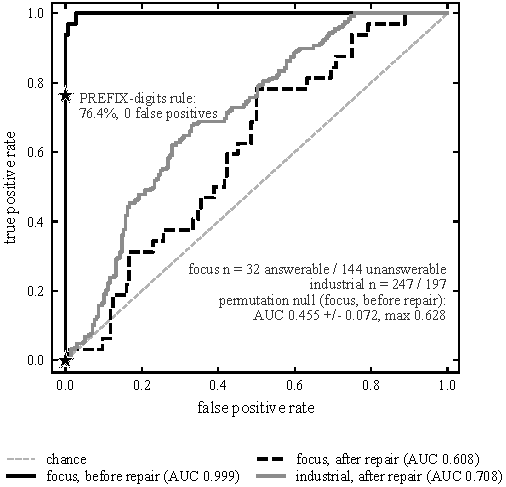
\includegraphics[width=0.72\textwidth]{figures/fig5_question_only_roc.pdf}
\caption{A classifier that sees only the question text --- no retrieval, no evidence, no corpus --- telling an answerable question from an unanswerable one, on both corpora and before and after the benchmark repair.}
\label{fig:fig5}
\end{figure}


\subsection{The retrieval findings replicate on authentic text}

The seven-rung ablation of Section~\ref{sec:results} was re-run unchanged on
the industrial corpus, over 247 answerable queries.
Table~\ref{tab:ind-ablation} gives the result and
Table~\ref{tab:ablation} the focus-corpus one.

\begin{table}[t]
\centering
\caption{Retrieval ablation on the industrial corpus: 247 answerable queries over 110 federal regulatory documents (2,443 chunks). Tbl R@10 is the recall over the table-bearing chunks only.}
\label{tab:ind-ablation}
\small
\begin{tabular}{lrrrrr}
\toprule
System & R@5 & R@10 & MRR & nDCG@10 & Tbl R@10 \\
\midrule
A. BM25 only & 0.8785 & 0.9595 & 0.7554 & 0.8026 & 0.969 \\
B. Dense only & 0.8300 & 0.8785 & 0.6600 & 0.7104 & 0.846 \\
C. Hybrid (RRF) & 0.9312 & 0.9595 & 0.7711 & 0.8160 & 0.946 \\
D. $+$ cross-encoder & 0.9757 & 0.9879 & 0.8269 & 0.8671 & 0.977 \\
E. $+$ category filter & 0.9717 & 0.9879 & 0.8339 & 0.8724 & 0.977 \\
F. $+$ quota (pre-rerank) & 0.9717 & 0.9798 & 0.8378 & 0.8740 & 0.985 \\
G. $+$ quota (post-rerank) & 0.9717 & 0.9879 & 0.8333 & 0.8724 & 0.977 \\
\bottomrule
\end{tabular}
\end{table}


The lexical leg carried the pipeline: BM25 reached
Recall@10 0.9595 against the dense
encoder's 0.8785, a difference of
-0.081 ($p=0.0003$, $n=247$).
That is a larger effect and a far smaller $p$ than the same comparison on the
focus corpus. It is also \emph{already published} --- lexical retrieval
beating an off-the-shelf dense encoder on legal and regulatory text has been
reported in several jurisdictions --- so it is not claimed here as new, and
the dense leg here is a general-purpose encoder that a domain-adapted one
could overtake. What the measurement contributes is the
\emph{corollary}: on this corpus neither the hybrid fusion
(+0.000, $p=1.0000$) nor the category
pre-filter (+0.000, $p=1.0000$) added
anything measurable on top of the lexical baseline. The cross-encoder did
help here (+0.028, $p=0.0196$), unlike on
the focus corpus.

The candidate-pool curve, which was saturated on the focus corpus and so
could not distinguish ``the pool stopped helping'' from ``the corpus had
nothing left to find'', is sharp here. At a pool of
50, Recall@20 reaches
1.000 while Recall@10 stands at
0.988: 1.21\% of the golds are retrieved
and then pushed \emph{out of the ten-chunk context} by the reranker's own
ordering. Enlarging the pool buys recall the context cannot hold.

The modality quota behaves as a trade on both corpora, and which way it
trades depends on where it is applied. Applied before the reranker it gives
up 0.8 points of overall recall
($p=0.3173$); applied after it, the industrial corpus
lands on exactly the no-quota operating point, with the pre-rerank arm at
Recall@10 0.9798 against the
post-rerank arm's 0.9879
(+0.008, $p=0.3173$).

\begin{figure}[t]
\centering
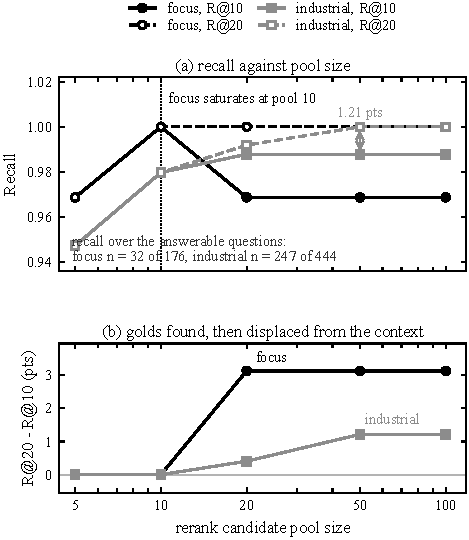
\includegraphics[width=0.72\textwidth]{figures/fig1_pool_size.pdf}
\caption{Recall against the size of the rerank candidate pool, on the focus corpus and on the industrial corpus.}
\label{fig:fig1}
\end{figure}


\begin{figure}[t]
\centering
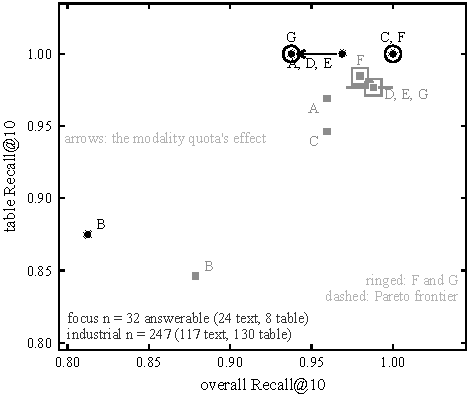
\includegraphics[width=0.72\textwidth]{figures/fig4_modality_quota_pareto.pdf}
\caption{Overall Recall@10 against table-specific Recall@10 for the seven ablated systems, on the focus corpus and on the industrial corpus.}
\label{fig:fig4}
\end{figure}


\subsection{The gate's operating point transfers; its threshold does not}

At $\tau = 0.40$ the industrial gate answers
91.5\% of the answerable queries and
refuses 58.9\% of the unanswerable
ones, with an abstention precision of 0.847 and
a coverage of 0.691. The threshold does not transfer ---
0.40 here against 0.05 on the focus corpus ---
and the operating point does: coverage 0.691 against
0.693. This is the calibration result of
Section~\ref{sec:results} restated on a second corpus: the threshold is a
fitted parameter of the deployment and must be re-fitted, while the point on
the risk--coverage surface a practitioner cares about is a property of the
mechanism. The two calibrations differ in quality as well as in value: the
industrial gate's expected calibration error is 0.075 against
0.104, while its Brier score is 0.159
against 0.151.

\begin{figure}[t]
\centering
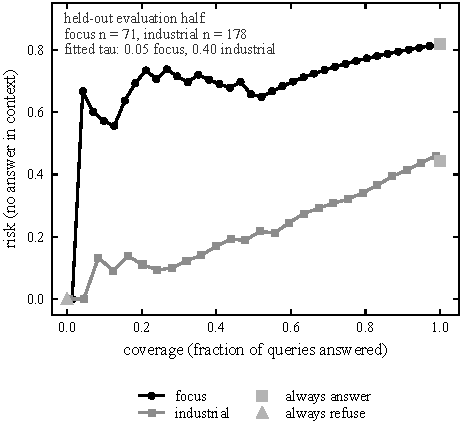
\includegraphics[width=0.72\textwidth]{figures/fig2_risk_coverage.pdf}
\caption{Risk--coverage of the confidence gate: the risk that an answered query has no answer in its context, against the fraction of queries the gate answers.}
\label{fig:fig2}
\end{figure}


\begin{figure}[t]
\centering
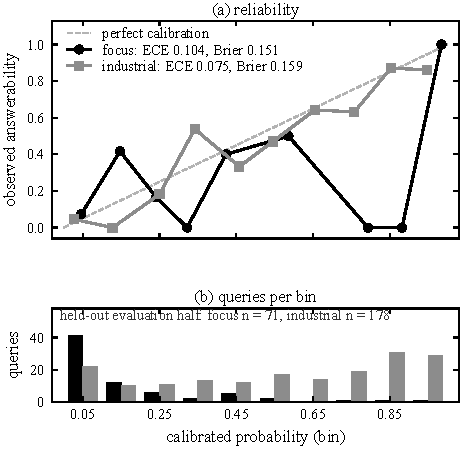
\includegraphics[width=0.72\textwidth]{figures/fig3_calibration.pdf}
\caption{Reliability of the gate's calibrated probability against observed answerability, on the held-out evaluation half of each corpus.}
\label{fig:fig3}
\end{figure}


\subsection{Detection and typing decompose}

This is the paper's clearest new result, and it needed a corpus that
contains conflicts to be visible.

240 pairs were assembled in two strata:
90 \emph{revision} pairs (a
paragraph and its amended self) and
150 \emph{similar} pairs
(cross-document retrieval neighbours). The pool is mined by the
\emph{retriever's} own lexical signal and never by the detector's numeric
rule, its NLI probability or its subject check: a pool selected on the
detector's decision rule cannot measure the detector's precision, because
every alarm would be in it by construction. The pairs were read by a panel of
domain specialists --- one per regulatory regime --- together with a
generalist control, all blind to the detector.

A conflict detector's precision is two numbers, not one.
\textbf{Detection} asks whether the alarm is pointing at something real.
\textbf{Typing} asks whether the branch that raised the alarm is the
branch that owns the conflict. Measured against the panel's labels, the
detector's detection precision is
0.659 (95\% CI
0.505--0.784)
and its typing precision is 0.073 (95\% CI
0.025--0.194).
On the stratum where the conflicts actually are, detection rises to
0.897.

Against the \emph{construction} labels --- the revision stratum, whose
conflict type is known without any judgement --- the separation is starker
still. Detection precision is 1.000:
every alarm the detector raises on that stratum points at a real conflict.
Typing precision is 0.000: not one alarm
was raised by the branch that owns its conflict. The semantic branch fired on
26 pairs, of which 24
were quantity conflicts; the revision branch fired on 3, of
which 3
were quantity conflicts; and the quantity branch fired on
0. Its recall against the
35 construction-labelled limit changes is
0.000.

So the mechanism \textbf{finds} the conflicts and \textbf{reports them as
the wrong kind}. It calls supersessions contradictions, and it cannot say
which version is in force --- because nothing in the retrieved passages says
which issue either of them is. On the industrial corpus the two branches are
also asymmetric in kind: the semantic branch accounts for
38 of the detector's alarms at a precision
against any real problem of
0.632, while
the revision branch accounts for 3 at
1.000. The
quantity branch is the thinnest result in the whole study: an exhaustive
corpus-wide search over 64 measurement terms found
1,776 candidate cross-document quantity
conflicts --- a count that is exact rather than sampled, because the search
groups every (measurement term, value) pair in the corpus and keeps the
terms whose values differ across documents --- of which
119 were put to the reader, and the branch fired on
13. The search is deliberately
over-inclusive: two passages about different boilers share the word
``pressure'', which is why the reader found
60 of the sampled pairs to be the same word
used for different things and none to be a genuine quantity conflict. The
branch's precision on this corpus is therefore not measurable, and the
framework's calibration floor would withhold it rather than report it.

\begin{figure}[t]
\centering
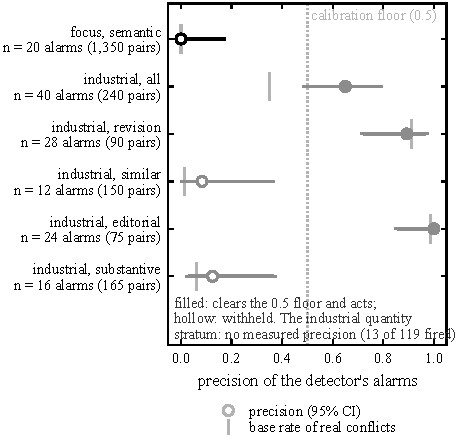
\includegraphics[width=0.72\textwidth]{figures/fig6_contradiction_precision.pdf}
\caption{The contradiction detector's precision against the base rate of real conflicts in the same population, with 95\% Wilson intervals; a filled marker clears the framework's 0.5 calibration floor and the branch would act, a hollow one does not.}
\label{fig:fig6}
\end{figure}


\subsection{The measurement's binding constraint was the rubric}

The comparison above was confounded, and the confound was in the
annotation rather than in the detector. The first comparison of the
old-rubric reader against the sharpened one had the same reader in one cell
and a different reader in the other, so ``the old rubric'' and ``the
generalist'' were the same cell. A $2\times2$ factorial separates them, with
the pairs, the detector and the regime briefs held constant.

\begin{table}[t]
\centering
\caption{The rubric $\times$ reader-specialisation factorial. Each cell is an independent reading of the same 240 pairs by the same detector, under the same regime briefs. Detection precision is the fraction of the reader's alarms that correspond to a real conflict; typing precision is the fraction raised by the branch that owns it. The lower block is the difference in detection precision between the two cells of each row and column.}
\label{tab:ind-factorial}
\small
\begin{tabular}{llrr}
\toprule
Reader & Rubric & Detection & Typing \\
\midrule
generalist & old (marker test) & 0.293 & 0.073 \\
generalist & sharpened (structural test) & 0.659 & 0.073 \\
specialist & old (marker test) & 0.341 & 0.073 \\
specialist & sharpened (structural test) & 0.659 & 0.073 \\
\bottomrule
\end{tabular}
\vspace{3pt}
\begin{tabular}{lr}
\toprule
Effect & $\Delta$ detection \\
\midrule
\emph{Rubric}, at the generalist & \textbf{+0.366} \\
\emph{Rubric}, at the specialist & \textbf{+0.317} \\
\emph{Specialisation}, at the old rubric & +0.049 \\
\emph{Specialisation}, at the sharpened rubric & +0.000 \\
\bottomrule
\end{tabular}
\end{table}


\emph{The rubric's wording moved the measured precision by about a third of
a point; the reader's domain specialisation moved it by almost nothing.}
The mechanism is concrete. The old rubric required a version marker, and a
regulation does not write its own version in its text, so it missed
63 of the
82 supersessions it was asked to find
(77\%),
calling them \texttt{no\_conflict}; the specialist reader missed
63 of
90
(70\%).

Three qualifications are owed to this result. First, the rubric changed the
\emph{definition} of the target as well as the procedure for recognising
one, and this experiment cannot separate the two; what it shows is that the
reader factor is small. Second, ``specialisation'' here was delivered as a
brief to a fixed reader model, not as a different capability, so the claim is
that a brief plus a sharpened rubric buys nothing over the rubric alone ---
narrower than ``specialists are not needed''. Third, the qualitative
principle is already published: that the annotation guideline is a
first-class error source in model annotation is established. What is new is
the factor of nine, and that it lands on the \emph{reported system
measurement} rather than only on the labels.

The generalisable lesson is about measurement rather than about annotation.
A number that moves by a factor of nine with the wording of its own rubric
is not yet a measurement of the thing under test.

\subsection{The per-claim band measures agreement, not correctness}

The third mechanism was measured on both corpora, with the same generator
that produced the focus corpus's answers and with two evidence protocols on
each: the benchmark's own gold evidence (is the claim right?) and the
evidence the retriever actually returned (does a reader agree with the
scorer?).

\begin{table}[t]
\centering
\caption{The per-claim confidence band against an independent reference, on both corpora and both evidence protocols. The kappa column is the agreement between the band and the reference on the binary question \emph{is this claim supported}. The band-error column gives the error rate of the \emph{grounded}, \emph{inferred} and \emph{uncertain} bands in that order. The last column is the share of answers containing no wrong claim, before and after keeping only the \emph{grounded} claims.}
\label{tab:ind-band}
\small
\begin{tabular}{lccc}
\toprule
Corpus and protocol & $\kappa$ & Band error (g/i/u) & Clean \\\midrule
Focus, gold & 0.049 (-0.026, +0.124) & 0.542 / 0.513 / 0.610 & 34.4\% $\rightarrow$ 50.0\% \\
Focus, retrieved & 0.069 (-0.002, +0.139) & 0.118 / 0.103 / 0.220 & 59.4\% $\rightarrow$ 81.2\% \\
Industrial, gold & 0.055 (-0.027, +0.138) & 0.077 / 0.119 / 0.139 & 91.1\% $\rightarrow$ 94.9\% \\
Industrial, retrieved & 0.017 (-0.066, +0.101) & 0.006 / 0.017 / 0.026 & 98.3\% $\rightarrow$ 99.6\% \\
\bottomrule
\end{tabular}
\end{table}


\emph{Caveat.} the focus corpus's gold protocol and the focus corpus's retrieved protocol were measured before the modality quota was moved to the other side of the cross-encoder, and the reference labels they rest on come from a panel of reader agents under a written protocol that could not be reproduced. They are quoted here as the earlier configuration's result.

Against an independent reference the band is at chance on all four
combinations: $\kappa$ 0.049 on the focus corpus's gold
evidence, 0.069 on its retrieved evidence, 0.055 on the
industrial corpus's gold evidence and 0.017 on its retrieved
evidence. The three bands are also indistinguishable on the gold protocols
(0.542 / 0.513 / 0.610 and
0.077 / 0.119 / 0.139), while they are
ordered on the evidence the band itself saw
(0.118 / 0.103 / 0.220 and
0.006 / 0.017 / 0.026). The sharper
way to state it: \textbf{the band measures whether the retrieved passages
entail the claim --- agreement with itself --- not whether the claim is
true.} As a filter it nonetheless works: keeping only the
\emph{grounded} claims raises the share of answers containing no wrong
claim from 34.4\% to 50.0\% on the focus corpus's
gold protocol, from 59.4\% to 81.2\% on its retrieved
protocol, and from 91.1\% to 94.9\% and
98.3\% to 99.6\% on the industrial corpus's two.

The positional comparison --- keeping the first half of an answer rather
than what the band tagged \emph{grounded} --- is the \emph{evidence} for
that reading, not the finding itself, and it does not hold everywhere. Of
the four corpus-and-protocol combinations, one gives a significant
positional result (the focus corpus's gold evidence,
$p=0.0081$, $d_z=+0.465$)
and three do not ($p=0.4174$, $p=1.0000$ and
$p=1.0000$). On the focus corpus's gold protocol the comparison is
also not a length artefact: later claims are \emph{shorter}
(Spearman $\rho$ -0.195,
$p=0.0003$).

\subsection{What the second corpus does not establish}

Five limits, stated rather than implied. One jurisdiction, one language and
one regulatory family: the corpus is US federal regulation, and nothing here
shows that the decomposition holds for a plant's own procedures, for a
non-English regulatory regime, or for a corpus of vendor specifications.
The labels are model-generated. The panel's agreement is reported in full,
but agreement between readers is not confirmation that a label is right, and
the thesis's own limitation table names this as the cost of replacing human
annotators. The positional comparison did not replicate across three of the
four combinations, so the band is reported as a filter with a measurement
decomposition, not as a ranking. The rubric factorial shows that the
annotation's wording moved the measurement, which is a warning about the
other measurements in this paper rather than a clean result about the
mechanism; and ``specialisation'' was a brief, not a capability. Finally, the
lexical-over-dense result is a boundary condition on \emph{this}
pipeline with a general-purpose encoder, not a claim about dense retrieval.
% END INDUSTRIAL-SECTION

\section{Discussion}

\subsection{What the framework does well}

Its strongest property is not any individual mechanism but that each is
\emph{structural}: the gate is a branch rather than an instruction, the quota is
enforced on the artefact the generator actually consumes, and the conflict
report is produced by an orthogonal conjunction rather than a single
classifier's opinion. In an industrial setting auditability is a functional
requirement --- a refusal whose reason can be reconstructed from a score and a
threshold is usable in a regulatory conversation, and one that cannot is not.
The second strength is the explicit separation of coverage from correctness as
quantities; a framework reporting a single hallucination rate has hidden the
trade-off. The third is the separation of \emph{detection} from \emph{typing}
in the contradiction gate: on the second corpus these are 0.659
against 0.073, and against labels whose conflict type is known
without judgement they are 1.000 against
0.000. A single precision number would have hidden
the more consequential of the two, which is that the mechanism finds real
conflicts and then reports them under the wrong label.

\subsection{What the framework does not do}

It does not resolve contradictions but surfaces them; given the published
conflict taxonomy, a type-tagged flag is the instrument available without a
trained conflict-type classifier, and the evidence suggests surfacing beats
resolution. On the second corpus it goes further and does not even say which
version of a superseded provision is in force, because nothing in the
retrieved passages carries the version: a detector for regulatory text needs
version metadata, or must be scoped to detection alone. It does not certify
its own confidence: the calibration is
empirical, on a held-out query split, under an exchangeability assumption that
a single-category industrial corpus violates. Nor does the form check parse
English: it is a lexical test, so it misses the malformed stems whose
malformation is grammatical rather than lexical --- truncated clauses such as
``what value is stated for assume customers arrive at the rate'' --- and it has
no dictionary or language model, so a keyboard mash passes it. It refuses
37.5\% of the hand-labelled malformed stems and fails open
on input it cannot judge, which is the conservative direction: a false
rejection would be a refusal of a question the corpus could have answered.
It does not beat long context on this corpus, and we measured both halves of that comparison. The most
serious threat is a 2026 study reporting long-context systems ahead of semantic
RAG in manufacturing safety, and on a 634-chunk corpus that baseline is
feasible. Three results bear on how it should be answered. The closest
published analogue to our corpus is favourable to retrieval:
Agri-Query~\cite{chen2026agriquery} places a 165-page agricultural-machinery
operator manual --- roughly 59K tokens, chunked at 200 tokens --- in the prompt
and reports that hybrid RAG consistently beats direct long context, with naive
insertion of the whole manual yielding significantly worse results. The
2025--2026 consensus is that the question is not \emph{which} to use but
\emph{when to route}: LaRA's title is literally \emph{No Silver Bullet for LC
or RAG Routing}~\cite{lu2025lara}, and the state of the art is a router that
escalates only the queries that need it --- our long-context arm is the
always-long-context arm of exactly that decision, and we measure it rather
than assert a preference for the other arm. Finally, \emph{Length Is Cheap,
Competition Is Not}~\cite{liu2026lengthcheap} reports that the attention mass
on evidence explains about 58\% of the variance in retrieval loss against at
most 8\% for log-length, and that a single competing value multiplies the loss
by 9--110x, so the expected way a whole-corpus prompt fails on industrial text
is competition among similar values rather than length as such.

MiniMax-M3 answered the same 32 answerable and 144 unanswerable questions behind five arms that share the generator, the prompt wording, the question set and the scorer, so a difference between them is attributable to the context and the gate and to nothing else: the same retrieval with the gate removed; the framework at the operating point fitted on this benchmark; a control that refuses as many questions as the fitted gate did, but picks them at random; the framework at the operating point transferred unchanged from the cross-category half; the whole corpus in the prompt. With the generator permitted to decline -- the deployed system -- The rate of answering the unanswerable questions was 0.535 (77 of 144), 0.417 (60 of 144), 0.375 (54 of 144), 0.014 (2 of 144), 0.528 (76 of 144) respectively, and the accuracy on the answerable ones 0.633 (30 of 32), 0.800 (30 of 32), 0.714 (21 of 32), 0.333 (6 of 32), 0.548 (31 of 32) respectively. With the permission to decline removed, and the model, the questions, the retrieval and the scorer all unchanged, The rate of answering the unanswerable questions was 0.938 (135 of 144), 0.528 (76 of 144), 0.604 (87 of 144), 0.021 (3 of 144), 0.931 (134 of 144) respectively, and the accuracy on the answerable ones 0.656 (32 of 32), 0.667 (30 of 32), 0.714 (21 of 32), 0.000 (6 of 32), 0.406 (32 of 32) respectively. Of the claims the arms produced on the unanswerable questions, the fraction supported by nothing in the evidence they were given was 0.554, 0.566, 0.529, 0.333, 0.548 respectively, on 130, 106, 85, 3, 155 claims A refusal that also asserts something -- the documents do not contain the demand for this SKU, so the quantity cannot be computed; in general it is computed as ... -- is counted as an answer and scored on the assertion, which is the reading that gives the gate less credit, and 48 of the unanswerable questions drew one. The claim scorer was audited against the benchmark before the comparison was read: 32 of the 33 answers the benchmark itself considers correct are recognised as supported by the evidence that states them, and 8 of the 9 fabricated values are rejected. The gate's contribution is measured under both prompt conditions, and it holds in both. Under the cautious prompt -- the deployed system -- the hypothesis is supported, at a price: the gate reduced the rate of answering unanswerable questions from 0.535 to 0.417, a fall of 11.8 points, at the cost of answering 30 of 32 answerable questions. Paired question by question, the gate refused 23 of the questions the ungated arm answered and let through 6 of the ones it did not (exact McNemar p = 0.002). Under the answering prompt, which differs from the cautious one by a single sentence and by nothing else, the hypothesis is supported, at a price: the gate reduced the rate of answering unanswerable questions from 0.938 to 0.528, a fall of 41.0 points, at the cost of answering 30 of 32 answerable questions. Paired question by question, the gate refused 60 of the questions the ungated arm answered and let through 1 of the ones it did not (exact McNemar p = < 0.001). What the framework claims is therefore not that the gate reduces hallucination whatever the generator does, but that it is the one component whose behaviour does not depend on the generator's cooperation: the prompt can be wrong, and the gate still holds. An audit of the benchmark's answer labels found that 27 of the 132 answerable questions carried an answer attached to the wrong question: a table question named the column its key came from while taking the answer from the next column, and some numeric golds were digit prefixes of longer tokens. The generator was corrected, the benchmark rebuilt and every experiment in this project re-measured against it, so the numbers reported here are post-repair; the audit now finds 0 defective labels out of 32, and the benchmark as it stood before the repair is kept so that the finding stays checkable. The accuracy margin over the long-context arm reaches no test's significance threshold -- not under the whole-answer entailment test, not under a length-controlled re-scoring of the same answers, and not under a lexical test that ignores length (p = 0.727, 0.508, 0.250), so the long-context comparison is settled on coverage and cost and directional rather than significant on answer quality.

\subsection{Threats to validity}

The principal internal threat is that the silver labels are optimistic and
mechanically tied to the chunking, which could inflate the benefit of a
retriever sharing the chunking's biases. The second internal threat is the
one this paper's own audit of its unanswerable class exposed and then
reduced: the class was separable from the question text alone, so the
pre-repair refusal rate was an upper bound, and a residual form-only effect
remains. The residual form-only separability of the repaired class is 0.608 against a permutation null of 0.468 (p = 0.050) on the focus domain, and 0.533 against a permutation null of 0.500 (p = 0.267) on the better-powered six-category benchmark. It is a small residual that the focus-domain run reaches and the better-powered run does not reproduce: small, but not zero. The repaired class is also labelled by the complement of the
benchmark's own extraction branches, and those branches are mechanical, so a
question the corpus answers in a form neither branch recognises is labelled
unanswerable when it is not. The rebuilt class is therefore a \emph{near-miss
class}: an independent re-check found 43 of 110 questions
whose subject the corpus comments on without
defining it, and 1 of 110 whose certificate does not hold at
all. The refusal rate is consequently measured on a class that is partly
answerable in a human's sense, which bounds what the absolute number means
without bounding the arm comparison, in which every arm is asked the same
questions; a hand-checked second annotation would settle the rest. The principal external threat is that
the corpus is public reference material rather than proprietary industrial
documentation, so the query distribution is not the operational one. The
second corpus narrows that threat but does not remove it: it is authentic,
binding and versioned, yet it is one jurisdiction, one language and one
regulatory family, and it is regulation rather than a plant's own procedures.
Three further threats are specific to it. The labels on the conflict pairs
are model-generated by a panel of domain specialists, so the panel's
agreement is reported in full, but agreement between readers is not
confirmation that a label is right; independent confirmation would require
human annotators. The wording of the annotation rubric moved the measured
precision by a factor of nine, which is a warning about every
model-annotated number in this paper and not only about that one. And the
positional comparison underlying the per-claim band does not replicate on
three of the four corpus-and-protocol combinations, so the band is reported
as a filter with a measurement decomposition rather than as a ranking. The
principal construct threat is that retrieval and gating quality are measured
but not end-to-end decision quality, which requires a practitioner study; the
16-participant pilot supports a within-subject sign test but not a claim about
generalisation. A second construct threat concerns the contradiction
mechanism specifically, whose precision has been measured against reader
labels rather than against a proxy: The contradiction gate's precision, measured against reader labels rather than against a proxy, is 0\%: none of the 20 labelled alarms was called a contradiction by either annotator, and the 95\% upper bound on the gate's true precision is 16.1\%. The two annotators do not share a model, both read the sheet blind to the detector's own scores, and both scored 14 of 14 on a control set whose labels are known in advance, and they agree on the contradiction/no-contradiction decision for 101 of the 101 pairs they labelled. The annotators are models rather than people, so the number says the alarms are not confirmed by a reader, not that no reader would ever confirm one.
 The detector's own positive control -- pairs whose correct behaviour is known in advance, written in the industrial register but not drawn from the corpus -- is 11 of 11, with every contradiction caught and every non-conflict left alone. So the mechanism works; this corpus does not test it.

\section{Conclusion}

This paper presented an evidence-grounded retrieval-augmented generation
framework for industrial decision support and was deliberate about the strength
of each kind of claim it makes. The architectural contribution is incremental
and is positioned against published prior art rather than asserted as priority.
The empirical contribution is a failure-mode characterisation: on an
independently constructed public industrial corpus, cross-encoder reranking is
shown to improve recall only when its candidate pool is an order of magnitude
larger than the final context; the modality quota is shown to bind only when
applied \emph{before} the reranker; the category pre-filter is shown to cost no
recall while improving the ordering, its benefit coming from restricting the
candidate pool the reranker sees rather than from reordering the fused ranking,
so that the soft-prior alternative proposed as its repair does not reproduce it;
and the modality composition of the corpus is
shown to determine whether a modality-aware mechanism can have any effect at
all. On a second corpus of versioned federal regulations, those negative
findings replicate --- the lexical leg carried the pipeline and neither the
fusion nor the pre-filter added anything measurable on top of it --- and the
candidate-pool curve stops being saturated, so that
1.21\% of the golds are retrieved and then displaced
out of the ten-chunk context. The clearest new result is a metric
contribution: a conflict detector's precision decomposes into detection and
typing, and on a corpus whose conflicts are known by construction the two are
1.000 and 0.000, so the
mechanism finds the conflicts and reports them as the wrong kind. A $2\times
2$ factorial then shows that the wording of the annotation rubric, not the
reader's domain specialisation, moved that measured precision, which is a
warning about the measurement rather than a clean result about the mechanism.
The methodological contribution is an evaluation protocol treating the
confidence gate as a selective-prediction policy with a risk--coverage curve
and a false-positive rate at a stated operating point, with always-flag and
never-flag baselines.

The framework's practical value does not depend on any mechanism being
individually novel. It depends on each being structural, on the trade-offs
between them being measured rather than assumed, and on the resulting system
being able to say, for every claim it makes, which passage supports it and how
confident the system is in that passage's relevance.

\section*{Data availability}
The corpus builder, benchmark generator, experiment scripts and full result
files (JSON and markdown) are released with this manuscript. The evaluation
corpus is fetched from public encyclopaedic endpoints and stored locally with a
manifest recording the source of every document, so that the corpus can be
rebuilt offline after the first fetch. The second corpus is fetched from the
Electronic Code of Federal Regulations versioner API, which serves any
regulation as it stood on any past date; the raw XML of both snapshots is
cached and the corpus, its manifest and the two benchmark files ship with the
manuscript. It is a work of the United States government and therefore in the
public domain. The six figures are released as PDF alongside the papers.

\section*{Reproducibility statement}
The corpus builder, benchmark generator, experiment scripts and full result
files are released with this manuscript. All stochastic components are seeded;
the index and embeddings are cached by content hash; and
the retrieval-side experiment scripts are deterministic given the seeds, while the generator-side comparison is not, because the generator's sampling temperature is provider-determined rather than seed-controlled; its five arms are therefore compared on rates over a fixed question set rather than on paired per-question outcomes. The complete measured tables underlying
every claim in Section~\ref{sec:results} are provided in machine-readable form
alongside the manuscript, and every arXiv identifier and DOI in the reference
list was resolved against a live bibliographic API.

\begin{thebibliography}{99}
\bibitem{lewis2020rag} P. Lewis, E. Perez, A. Piktus, F. Petroni, V. Karpukhin, N. Goyal, H. K\"uttler, M. Lewis, W. Yih, T. Rockt\"aschel, S. Riedel, and D. Kiela, ``Retrieval-augmented generation for knowledge-intensive NLP tasks,'' in \emph{NeurIPS}, 2020, pp. 9459--9474.
\bibitem{karpukhin2020dpr} V. Karpukhin, B. Oguz, S. Min, P. Lewis, L. Wu, S. Edunov, D. Chen, and W. Yih, ``Dense passage retrieval for open-domain question answering,'' in \emph{EMNLP}, 2020, pp. 6769--6781.
\bibitem{asai2024selfrag} A. Asai, Z. Wu, Y. Wang, A. Sil, and H. Hajishirzi, ``Self-RAG: Learning to retrieve, generate, and critique through self-reflection,'' in \emph{ICLR}, 2024.
\bibitem{yan2024crag} S.-Q. Yan, J.-C. Gu, Y. Zhu, and Z.-H. Ling, ``Corrective retrieval augmented generation,'' 2024. [Online]. Available: arXiv:2401.15884
\bibitem{jiang2023flare} Z. Jiang, F. F. Xu, L. Gao, Z. Sun, Q. Liu, J. Dwivedi-Yu, Y. Yang, J. Callan, and G. Neubig, ``Active retrieval augmented generation,'' in \emph{EMNLP}, 2023.
\bibitem{su2024dragin} W. Su, Y. Tang, Q. Ai, and Z. Wu, ``DRAGIN: Dynamic retrieval augmented generation based on the real-time information needs of large language models,'' in \emph{ACL}, 2024.
\bibitem{jeong2024adaptive} S. Jeong, J. Baek, S. Cho, and S. J. Hwang, ``Adaptive-RAG: Learning to adapt retrieval-augmented LLMs through question complexity,'' in \emph{NAACL}, 2024.
\bibitem{rajpurkar2018squad2} P. Rajpurkar, R. Jia, and P. Liang, ``Know what you don't know: Unanswerable questions for SQuAD,'' in \emph{ACL}, 2018, pp. 518--528.
\bibitem{kadavath2022know} S. Kadavath, T. Conerly, A. Askell, and T. Henighan, ``Language models (mostly) know what they know,'' 2022. [Online]. Available: arXiv:2207.05221
\bibitem{kuhn2023semantic} L. Kuhn, Y. Gal, and S. Farquhar, ``Semantic uncertainty: Linguistic invariances for uncertainty estimation in natural language generation,'' in \emph{ICLR}, 2023.
\bibitem{farquhar2024semantic} S. Farquhar, J. Kossen, L. Kuhn, and Y. Gal, ``Detecting hallucinations in large language models using semantic entropy,'' \emph{Nature}, vol. 630, no. 8015, pp. 625--630, 2024.
\bibitem{joren2024sufficient} H. Joren, J. Zhang, C.-S. Ferng, D.-C. Juan, and A. Taly, ``Sufficient context: A new lens on retrieval augmented generation systems,'' 2024. [Online]. Available: arXiv:2411.06037
\bibitem{geissler2026dependable} F. Gei{\ss}ler, F. Carella, L. Fieback, and J. Spiegelberg, ``Towards dependable retrieval-augmented generation using factual confidence prediction,'' 2026. [Online]. Available: arXiv:2605.05244
\bibitem{phillips2026entropy} E. Phillips, F. Gustafsson, S. Wu, A. Thakur, and D. A. Clifton, ``Entropy alone is insufficient for safe selective prediction in LLMs,'' 2026. [Online]. Available: arXiv:2603.21172
\bibitem{thakur2026declinecraft} A. Thakur, A. Saparov, and B. Ribeiro, ``DeclineCraft: A RAG abstention benchmark for jointly measuring combined retrieval and parametric knowledge,'' 2026. [Online]. Available: arXiv:2610.28340
\bibitem{yadkori2024conformal} Y. A. Yadkori, I. Kuzborskij, D. Stutz, and A. Gy\"orgy, ``Mitigating LLM hallucinations via conformal abstention,'' 2024. [Online]. Available: arXiv:2405.01563
\bibitem{faysse2025colpali} M. Faysse, H. Sibille, T. Wu, B. Omrani, G. Viaud, C. Hudelet, and P. Colombo, ``ColPali: Efficient document retrieval with vision language models,'' in \emph{ICLR}, 2025.
\bibitem{suri2024visdom} M. Suri, P. Mathur, F. Dernoncourt, et al., ``VisDoM: Multi-document QA with visually rich elements using multimodal retrieval-augmented generation,'' 2024. [Online]. Available: arXiv:2412.10704
\bibitem{strich2026t2} J. Strich, E. K. Isgorur, M. Trescher, et al., ``T2-RAGBench: Text-and-table benchmark for evaluating retrieval-augmented generation,'' in \emph{EACL}, 2026.
\bibitem{thakur2021beir} N. Thakur, N. Reimers, A. R\"uckl\'e, et al., ``BEIR: A heterogeneous benchmark for zero-shot evaluation of information retrieval models,'' in \emph{NeurIPS Datasets and Benchmarks}, 2021.
\bibitem{decian2026dynamic} J. Decian, C. Njeh, and H. Nakouri, ``Dynamic RAG with hybrid retrieval: A novel approach to robust LLMs and hallucination prevention,'' \emph{Neurocomputing}, vol. 705, art. 134911, 2026. https://doi.org/10.1016/j.neucom.2026.134911
\bibitem{gao2023alce} T. Gao, H. Yen, J.-T. Yu, and D. Chen, ``Enabling large language models to generate text with citations,'' in \emph{EMNLP}, 2023.
\bibitem{chen2026principled} Y. Chen, et al., ``Principled context engineering for RAG: Statistical guarantees via conformal prediction,'' in \emph{ECIR}, 2026. [Online]. Available: arXiv:2511.17908
\bibitem{longcontext2026tokentax} ``The token tax of epistemic accuracy: Comparing RAG and long-context architectures for document-grounded generative AI applications,'' 2026. [Online]. Available: arXiv:2606.20898
\bibitem{ranking2026notdeciding} ``Ranking is not deciding: Benchmark shortcuts and operating-point collapse in query-time RAG poisoning defenses,'' 2026. [Online]. Available: arXiv:2610.33849
\bibitem{claimconformal2026} ``Claim-level conformal prediction for retrieval-augmented generation,'' 2026. [Online]. Available: arXiv:2610.34872
\bibitem{syncheck2024} D. Wu, J.-C. Gu, F. Yin, and N. Peng, ``Synchronous faithfulness monitoring for trustworthy retrieval-augmented generation,'' in \emph{EMNLP}, 2024, pp. 9390--9406. [Online]. Available: \url{https://doi.org/10.18653/v1/2024.emnlp-main.527}
\bibitem{es2024ragas} S. Es, J. James, L. Espinosa-Anke, and S. Schockaert, ``RAGAS: Automated evaluation of retrieval augmented generation,'' in \emph{EACL System Demonstrations}, 2024.
\bibitem{saadfalcon2024ares} J. Saad-Falcon, O. Khattab, C. Potts, et al., ``ARES: An automated evaluation framework for retrieval-augmented generation systems,'' in \emph{NAACL}, 2024.
\bibitem{min2023factscore} S. Min, K. Krishna, X. Lyu, et al., ``FActScore: Fine-grained atomic evaluation of factual precision in long form text generation,'' in \emph{EMNLP}, 2023.
\bibitem{williams2018mnli} A. Williams, N. Nangia, P. Bowman, et al., ``An extensive evaluation of the natural language inference task,'' in \emph{ACL}, 2018.
\bibitem{nie2020anli} Y. Nie, A. H. Zhou, R. Socher, and J. Gao, ``ANLI: Annotating adversarially with natural language inference,'' in \emph{ACL}, 2020.
\bibitem{yang2026contextconflict} X. Yang, Z. Liu, R. Li, et al., ``Large language models in resolving contextual knowledge conflicts,'' in \emph{EMNLP}, 2026, pp. 21142--21169.
\bibitem{liu2026conflictscore} S. Liu, A. Halfaker, D. Roth, et al., ``ConflictScore: Identifying and measuring how language models handle conflicting evidence,'' in \emph{EMNLP}, 2026, pp. 58825--58845.
\bibitem{feng2025conformal} N. Feng, Y. Sui, S. Hou, et al., ``Response quality assessment for retrieval-augmented generation via conditional conformal factuality,'' in \emph{SIGIR}, 2025.
\bibitem{yi2026grace} J. S. K. Yi, J. Minot, D.-Y. Lee, et al., ``GRACE: Graph-grounded reflective agent copilot engine for expert-in-the-loop knowledge expansion,'' 2026. [Online]. Available: arXiv:2609.04442
\bibitem{jang2025calibrag} C. Jang, D. Cho, S. Lee, H. Lee, and J. Lee, ``Reliable decision making via calibration oriented retrieval augmented generation,'' in \emph{NeurIPS}, 2025.
\bibitem{cormack2009rrf} G. V. Cormack, C. L. A. Clarke, and S. B\"uttcher, ``Reciprocal rank fusion outperforms Condorcet and individual rank learning methods,'' in \emph{SIGIR}, 2009, pp. 758--759.
\bibitem{bruch2023fusion} S. Bruch, S. Gai, and A. Ingber, ``An analysis of fusion functions for hybrid retrieval,'' \emph{ACM Trans. Inf. Syst.}, vol. 41, no. 6, 2023.
\bibitem{robertson2004prf} S. Robertson, H. Zaragoza, and J. Taylor, ``Probabilistic relevance framework: BM25 and beyond,'' \emph{Found. Trends Inf. Retr.}, vol. 3, no. 4, pp. 333--389, 2004.
\bibitem{huang2024selfcorrect} J. Huang, X. Chen, S. R. Mishra, H. Zheng, A. Chandak, Y. Wu, and X. Li, ``Large language models cannot self-correct reasoning yet,'' in \emph{ICLR}, 2024.
\bibitem{goswami2025haltrag} S. Goswami and S. Kurra, ``HALT-RAG: A task-adaptable framework for hallucination detection with calibrated NLI ensembles and abstention,'' 2025. [Online]. Available: arXiv:2509.07475
\bibitem{zong2026icalm} Y. Zong, Y. Li, X. Long, L. Chang, T. Wu, and R. Hadfield, ``I-CALM: Incentivizing confidence-aware abstention for LLM selective answering,'' 2026. [Online]. Available: arXiv:2604.03904
\bibitem{zhang2026taps} Y. Zhang, S. Wang, L. Yang, H. Tan, L. Tang, Y. Chen, L. Wang, and M. Sun, ``Strong yet controllable LLM abstention without learning to abstain,'' 2026. [Online]. Available: arXiv:2610.16318
\bibitem{peng2025uaeval4rag} T. Peng, S. Choubey, X. Xiong, and W. Wu, ``Unanswerability evaluation for retrieval augmented generation,'' in \emph{ACL}, 2025. [Online]. Available: \url{https://aclanthology.org/2025.acl-long.415/}
\bibitem{tikhomirov2026selection} A. Tikhomirov and V. Savchenko, ``The selection effect: Why compact LLM verifiers for emotion classification fail behind encoder confidence gates,'' in \emph{EMNLP}, 2026. [Online]. Available: \url{https://aclanthology.org/2026.emnlp-main.1049/}
\bibitem{du2026recognition} S. Du and L. Hu, ``Recognition--refusal misalignment in LLMs: Why models answer structurally unanswerable questions,'' in \emph{EMNLP}, 2026. [Online]. Available: \url{https://aclanthology.org/2026.emnlp-main.1078/}
\bibitem{cocchieri2026overcommit} E. Cocchieri, L. Ragazzi, M. Tagliavini, and M. Moro, ``LLMs (almost) never abstain under medical uncertainty,'' in \emph{ACL}, 2026. [Online]. Available: \url{https://aclanthology.org/2026.acl-long.1365/}
\bibitem{chen2026agriquery} ``Agri-Query: A case study on RAG vs. long-context LLMs for cross-lingual technical question answering,'' 2025. [Online]. Available: arXiv:2508.18093
\bibitem{lu2025lara} ``LaRA: Benchmarking retrieval-augmented generation and long-context LLMs --- no silver bullet for LC or RAG routing,'' 2025. [Online]. Available: arXiv:2502.09977
\bibitem{liu2026lengthcheap} ``Length is cheap, competition is not: Attention predicts context rot in retrieval,'' 2026. [Online]. Available: arXiv:2611.04169
\bibitem{rosario2026jev} S. Do Rosario and M. Atef, ``Jev-as-a-judge for RAG claim verification: Confidence-gated cascading between a non-generative verifier and a frontier LLM,'' 2026. [Online]. Available: arXiv:2610.20634
\bibitem{ravuri2026rcl} ``RCL: A retrieval-confidence layer for detecting insufficient context in enterprise retrieval-augmented code generation,'' 2026. [Online]. Available: arXiv:2609.11023
\bibitem{zheng2026citeguard} ``CiteGuard-RAG: A validation-centered AI system for evidence-grounded question answering,'' 2026. [Online]. Available: arXiv:2609.15830
\bibitem{tian2026hira} Y. Tian, X. Chen, and L. Queiroz, ``HIRA: A human-in-the-loop retrieval-augmented cascade for document classification in regulated industries,'' in \emph{CIKM}, 2026. [Online]. Available: arXiv:2608.21792
\bibitem{chen2026modalityutility} ``Modality relevance is not modality utility: Post-hoc selective modality escalation for cost-aware multimodal RAG,'' 2026. [Online]. Available: arXiv:2607.05438
\bibitem{sharma2026placebo} ``Does document structure help dense retrieval? A placebo-controlled ablation of four mechanisms across two corpora,'' 2026. [Online]. Available: arXiv:2610.10170

\bibitem{yang2024ehrsql} Y. Yang, S. Kim, S. Kim, G. Lee, S.-Y. Yun, and E. Choi, ``Towards unbiased evaluation of detecting unanswerable questions in EHRSQL,'' 2024. [Online]. Available: arXiv:2405.01588
\bibitem{mondal2026beforeanswering} J. J. Mondal, M. S. A. Apurba, M. Banik, M. M. Al Mahmud, and I. F. Shihab, ``Before answering: Evidence sufficiency under size-matched memory construction,'' 2026. [Online]. Available: arXiv:2609.32269
\bibitem{brunello2026folio} A. Brunello, C. Curaba, L. Geatti, M. Mignani, A. Montanari, and N. Saccomanno, ``Fixing FOLIO and MALLS: Verified annotations and an LLM-assisted framework to focus human relabeling,'' 2026. [Online]. Available: arXiv:2606.02837
\bibitem{gautam2023unanswerable} V. Gautam, M. Zhang, and D. Klakow, ``A lightweight method to generate unanswerable questions in English,'' in \emph{Findings of EMNLP}, 2023. [Online]. Available: arXiv:2310.19403
\bibitem{semnani2025wikicollide} S. J. Semnani, J. Burapacheep, A. Khatua, et al., ``Detecting corpus-level knowledge inconsistencies in Wikipedia with large language models,'' in \emph{EMNLP}, 2025. [Online]. Available: arXiv:2509.23233
\bibitem{won2026sievesage} J. Won, S. G. An, and J.-Y. Lee, ``Sieve and Sage: Efficient distraction filtering for reliable RALM abstention,'' in \emph{Findings of EMNLP}, 2026. [Online]. Available: arXiv:2609.35794
\bibitem{li2026relevance} Y. Li, S. Li, Z. Xu, et al., ``Relevance is not sufficiency: What actually closes the evidence gap in long-term memory QA,'' 2026. [Online]. Available: arXiv:2610.09348
\bibitem{setiawan2026grabrag} Y. A. Setiawan, ``Prompt-based abstention fails under misleading context: A controlled study of small frozen RAG models,'' in \emph{AACL-IJCNLP}, 2026. [Online]. Available: arXiv:2608.22228
\bibitem{ling2026promptartifact} Z. Ling, S. Liu, Y. Tang, et al., ``LLM abstention can be a prompt artifact, in addition to genuine uncertainty,'' in \emph{EMNLP}, 2026, pp. 12612--12633. [Online]. Available: \url{https://doi.org/10.18653/2026.emnlp-main.549}
\bibitem{singh2026beyondreranker} S. Singh, A. Reddy, and M. Chopra, ``Beyond the reranker: Do RAG retrieval enhancements help once a strong reranker is present?'' 2026. [Online]. Available: arXiv:2606.28367
\bibitem{zhou2026crowding} Y. Zhou, J. Yin, F. Zhang, et al., ``Financial evidence crowding: Diagnosing and mitigating constraint-induced displacement in retrieval-augmented generation,'' 2026. [Online]. Available: arXiv:2609.35782
\bibitem{zhang2026certify} X. Zhang and W. Sun, ``Knowing when the evidence is enough: Requirement-directed search with Horn-closure certificates,'' 2026. [Online]. Available: arXiv:2610.34684
\bibitem{qiu2026surerag} J. Qiu, Z. Han, and C. Huang, ``SURE-RAG: Sufficiency and uncertainty-aware evidence verification for selective retrieval-augmented generation,'' 2026. [Online]. Available: arXiv:2605.03534
\bibitem{knafou2026bitem} J. Knafou, L. Mottin, A. Flament, et al., ``BITEM at the NTCIR-19 R2C2 task: Predicting confidence from agentic RAG pipeline signals,'' 2026. [Online]. Available: arXiv:2609.37993
\bibitem{wei2026kontrast} F. Wei, T. Ehrhart, and R. Troncy, ``Detecting knowledge inconsistencies across text, tables, and knowledge graphs,'' 2026. [Online]. Available: arXiv:2607.25959
\bibitem{an2026fresco} S. An, H. Lee, S. Yuan, et al., ``FRESCO: Benchmarking and optimizing re-rankers for evolving semantic conflict in retrieval-augmented generation,'' 2026. [Online]. Available: arXiv:2604.14227
\bibitem{valjakka2026labeling} J. Valjakka, J. Kivim\"aki, J. Myll\"ari, and J. K. Nurminen, ``The labeling problem in hallucination detection benchmarks: An empirical evaluation,'' in \emph{NeurIPS Datasets and Benchmarks}, 2026. [Online]. Available: arXiv:2610.08026
\bibitem{singh2025manufacturing} R. Singh, A. Hamilton, A. White, et al., ``A multimodal manufacturing safety chatbot: Knowledge base design, benchmark development, and evaluation of multiple RAG approaches,'' 2025. [Online]. Available: arXiv:2511.11847
\bibitem{khalid2026automotive} M. Khalid and Y. Uygun, ``An industrial-scale retrieval-augmented generation framework for requirements engineering: Empirical evaluation with automotive manufacturing data,'' 2026. [Online]. Available: arXiv:2603.20534
\bibitem{solodko2026lakequest} M. Solodko, S. Gong, G. Yu, et al., ``LakeQuest: A three-domain benchmark for grounded question answering across data lakes,'' in \emph{COLM}, 2026. [Online]. Available: arXiv:2607.12310
\bibitem{joshi2026realdocbench} A. Joshi, J. Kim, G. Eggert, et al., ``RealDocBench: A benchmark for field-level QA and layout understanding on real-world regulated documents,'' 2026. [Online]. Available: arXiv:2606.07401
\bibitem{qian2026fabbench} J. Qian, C. Yi, M. Xia, et al., ``FAB-Bench: A framework for adaptive RAG benchmarking in semiconductor manufacturing,'' 2026. [Online]. Available: arXiv:2605.26476
\bibitem{park2026induspecqa} J. Park, H. Jeon, Y. Lee, and M. Kim, ``Ontology-based knowledge graphs for industrial standards with scope-aware logical rule structuring,'' in \emph{EMNLP}, 2026, pp. 33282--33311. [Online]. Available: \url{https://doi.org/10.18653/2026.emnlp-main.1456}
\bibitem{bruckhaus2024ragenterprises} T. Bruckhaus, ``RAG does not work for enterprises,'' 2024. [Online]. Available: arXiv:2406.04369
\bibitem{faria2026clairfin} F. T. J. Faria, M. B. Moin, J. A. Mahmud, et al., ``CLAIR-Fin: An adversarial multi-agent framework for claim-level verification and adaptive debate in cross-modal financial QA,'' in \emph{FinNLP}, 2026. [Online]. Available: arXiv:2608.13706
\bibitem{mori2025lexical} L. Mori, C. S. de Oliveira, Y. Yih, and M. Ventresca, ``Assessing the performance gap between lexical and semantic models for information retrieval with formulaic legal language,'' 2025. [Online]. Available: arXiv:2506.12895
\bibitem{lotfi2024bsard} E. Lotfi, N. Banar, N. Yuzbashyan, and W. Daelemans, ``Bilingual BSARD: Extending statutory article retrieval to Dutch,'' in \emph{RegNLP}, 2025. [Online]. Available: arXiv:2412.07462
\bibitem{pereira2026jua} J. Pereira, L. Fernandes, E. de Brito, R. Lotufo, and L. Bonifacio, ``JU\'A --- a benchmark for information retrieval in Brazilian legal text collections,'' 2026. [Online]. Available: arXiv:2604.06098
\bibitem{akarsu2026bm25} M. Akarsu, R. K. Karaman, and C. Mierbach, ``From BM25 to corrective RAG: Benchmarking retrieval strategies for text-and-table documents,'' 2026. [Online]. Available: arXiv:2604.01733
\bibitem{wang2026bm25scale} P. Wang, B. Xu, S. Wang, M. Du, X. Zeng, H. Wu, L. Zhang, and L. Zhang, ``BM25 wins at scale: A scaling study of retrieval-augmented generation paradigms,'' 2026. [Online]. Available: arXiv:2607.26497
\bibitem{beta2026greekbar} E. Beta, O. S. Chlapanis, D. Galanis, and I. Androutsopoulos, ``GreekBarRetrieval: A benchmark for Greek statutory retrieval,'' in \emph{NLLP}, 2026. [Online]. Available: arXiv:2608.18752
\bibitem{gajjar2026teleembed} P. Gajjar and V. K. Shah, ``TeleEmbedBench: A multi-corpus embedding benchmark for RAG in telecommunications,'' 2026. [Online]. Available: arXiv:2604.17778
\bibitem{cheng2024silicon} X. Cheng, R. Mayya, and J. Sedoc, ``To err is human; to annotate, SILICON? Toward robust reproducibility in LLM annotation,'' 2024. [Online]. Available: arXiv:2412.14461
\bibitem{kim2026guidelines} K. W. Kim, J.-D. Kim, and A. Aizawa, ``Refining and reusing annotation guidelines for LLM annotation,'' in \emph{ACL}, 2026. [Online]. Available: arXiv:2605.20809
\bibitem{akarajaradwong2026nitibench} P. Akarajaradwong, S. Nutanong, and C. Chaksangchaichot, ``NitiBench+: A temporal Thai legal question answering benchmark across 17 domains,'' 2026. [Online]. Available: arXiv:2611.03576
\bibitem{prior2026oldfriend} M. Prior, A. Schultz, and M. Grabmair, ``Asking for an old friend: Diagnosing and mitigating temporal failure modes in LLM-based statutory question answering,'' in \emph{ICAIL}, 2026. [Online]. Available: arXiv:2605.23497
\bibitem{huang2026wronglaw} Y. Huang, Y. Zhou, Q. Liu, S. Peng, Y. Kong, K. Funakoshi, C. Xiao, M. Okumura, Y. Cao, and S. Zheng, ``When do LLMs apply the wrong law? Diagnosing LLM failures in temporal legal reasoning,'' 2026. [Online]. Available: arXiv:2608.14610
\bibitem{yu2026detecting} Z. Yu, W. Xing, C. Ye, X. Teng, B. Yang, C. Lin, and M. Han, ``Detecting is not resolving: The monitoring control gap in retrieval augmented LLMs,'' 2026. [Online]. Available: arXiv:2605.27157
\bibitem{cattan2025dragged} A. Cattan, A. Jacovi, O. Ram, J. Herzig, R. Aharoni, S. Goldshtein, E. Ofek, I. Szpektor, and A. Caciularu, ``DRAGged into conflicts: Detecting and addressing conflicting sources in search-augmented LLMs,'' 2025. [Online]. Available: arXiv:2506.08500
\bibitem{rehman2026conformal} M. A. Rehman and C.-K. Yeh, ``Conformal factuality control for multi-hop retrieval-augmented generation,'' 2026. [Online]. Available: arXiv:2609.38222
\end{thebibliography}

\end{document}
